\documentclass[1p]{elsarticle_modified}
%\bibliographystyle{elsarticle-num}

%\usepackage[colorlinks]{hyperref}
%\usepackage{abbrmath_seonhwa} %\Abb, \Ascr, \Acal ,\Abf, \Afrak
\usepackage{amsfonts}
\usepackage{amssymb}
\usepackage{amsmath}
\usepackage{amsthm}
\usepackage{scalefnt}
\usepackage{amsbsy}
\usepackage{kotex}
\usepackage{caption}
\usepackage{subfig}
\usepackage{color}
\usepackage{graphicx}
\usepackage{xcolor} %% white, black, red, green, blue, cyan, magenta, yellow
\usepackage{float}
\usepackage{setspace}
\usepackage{hyperref}

\usepackage{tikz}
\usetikzlibrary{arrows}

\usepackage{multirow}
\usepackage{array} % fixed length table
\usepackage{hhline}

%%%%%%%%%%%%%%%%%%%%%
\makeatletter
\renewcommand*\env@matrix[1][\arraystretch]{%
	\edef\arraystretch{#1}%
	\hskip -\arraycolsep
	\let\@ifnextchar\new@ifnextchar
	\array{*\c@MaxMatrixCols c}}
\makeatother %https://tex.stackexchange.com/questions/14071/how-can-i-increase-the-line-spacing-in-a-matrix
%%%%%%%%%%%%%%%

\usepackage[normalem]{ulem}

\newcommand{\msout}[1]{\ifmmode\text{\sout{\ensuremath{#1}}}\else\sout{#1}\fi}
%SOURCE: \msout is \stkout macro in https://tex.stackexchange.com/questions/20609/strikeout-in-math-mode

\newcommand{\cancel}[1]{
	\ifmmode
	{\color{red}\msout{#1}}
	\else
	{\color{red}\sout{#1}}
	\fi
}

\newcommand{\add}[1]{
	{\color{blue}\uwave{#1}}
}

\newcommand{\replace}[2]{
	\ifmmode
	{\color{red}\msout{#1}}{\color{blue}\uwave{#2}}
	\else
	{\color{red}\sout{#1}}{\color{blue}\uwave{#2}}
	\fi
}

\newcommand{\Sol}{\mathcal{S}} %segment
\newcommand{\D}{D} %diagram
\newcommand{\A}{\mathcal{A}} %arc


%%%%%%%%%%%%%%%%%%%%%%%%%%%%%5 test

\def\sl{\operatorname{\textup{SL}}(2,\Cbb)}
\def\psl{\operatorname{\textup{PSL}}(2,\Cbb)}
\def\quan{\mkern 1mu \triangleright \mkern 1mu}

\theoremstyle{definition}
\newtheorem{thm}{Theorem}[section]
\newtheorem{prop}[thm]{Proposition}
\newtheorem{lem}[thm]{Lemma}
\newtheorem{ques}[thm]{Question}
\newtheorem{cor}[thm]{Corollary}
\newtheorem{defn}[thm]{Definition}
\newtheorem{exam}[thm]{Example}
\newtheorem{rmk}[thm]{Remark}
\newtheorem{alg}[thm]{Algorithm}

\newcommand{\I}{\sqrt{-1}}
\begin{document}

%\begin{frontmatter}
%
%\title{Boundary parabolic representations of knots up to 8 crossings}
%
%%% Group authors per affiliation:
%\author{Yunhi Cho} 
%\address{Department of Mathematics, University of Seoul, Seoul, Korea}
%\ead{yhcho@uos.ac.kr}
%
%
%\author{Seonhwa Kim} %\fnref{s_kim}}
%\address{Center for Geometry and Physics, Institute for Basic Science, Pohang, 37673, Korea}
%\ead{ryeona17@ibs.re.kr}
%
%\author{Hyuk Kim}
%\address{Department of Mathematical Sciences, Seoul National University, Seoul 08826, Korea}
%\ead{hyukkim@snu.ac.kr}
%
%\author{Seokbeom Yoon}
%\address{Department of Mathematical Sciences, Seoul National University, Seoul, 08826,  Korea}
%\ead{sbyoon15@snu.ac.kr}
%
%\begin{abstract}
%We find all boundary parabolic representation of knots up to 8 crossings.
%
%\end{abstract}
%\begin{keyword}
%    \MSC[2010] 57M25 
%\end{keyword}
%
%\end{frontmatter}

%\linenumbers
%\tableofcontents
%
\newcommand\colored[1]{\textcolor{white}{\rule[-0.35ex]{0.8em}{1.4ex}}\kern-0.8em\color{red} #1}%
%\newcommand\colored[1]{\textcolor{white}{ #1}\kern-2.17ex	\textcolor{white}{ #1}\kern-1.81ex	\textcolor{white}{ #1}\kern-2.15ex\color{red}#1	}

{\Large $\underline{12a_{1092}~(K12a_{1092})}$}

\setlength{\tabcolsep}{10pt}
\renewcommand{\arraystretch}{1.6}
\vspace{1cm}\begin{tabular}{m{100pt}>{\centering\arraybackslash}m{274pt}}
\multirow{5}{120pt}{
	\centering
	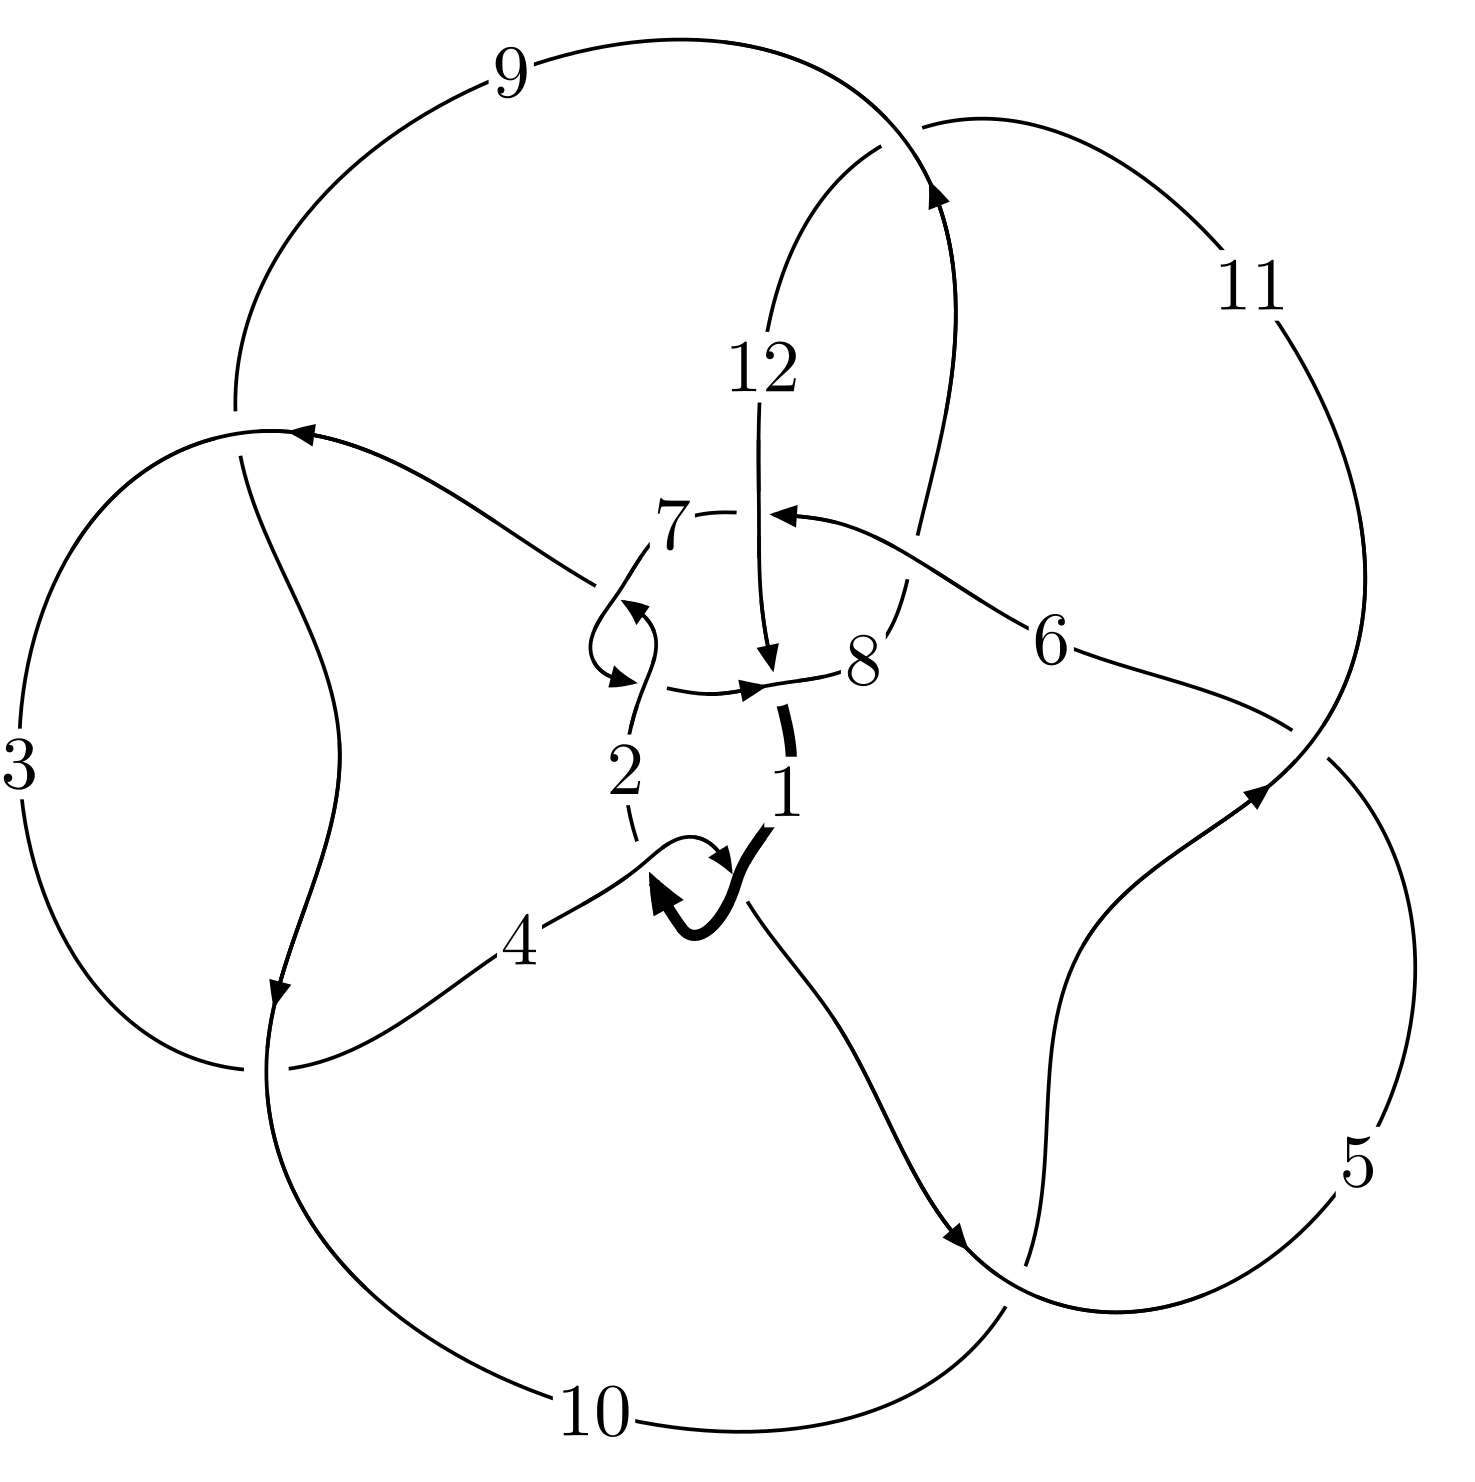
\includegraphics[width=112pt]{../../../GIT/diagram.site/Diagrams/png/1893_12a_1092.png}\\
\ \ \ A knot diagram\footnotemark}&
\allowdisplaybreaks
\textbf{Linearized knot diagam} \\
\cline{2-2}
 &
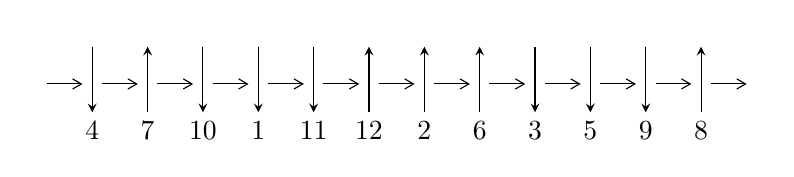
\begin{tikzpicture}[x=20pt, y=17pt]
	% nodes
	\node (C0) at (0, 0) {};
	\node (C1) at (1, 0) {};
	\node (C1U) at (1, +1) {};
	\node (C1D) at (1, -1) {4};

	\node (C2) at (2, 0) {};
	\node (C2U) at (2, +1) {};
	\node (C2D) at (2, -1) {7};

	\node (C3) at (3, 0) {};
	\node (C3U) at (3, +1) {};
	\node (C3D) at (3, -1) {10};

	\node (C4) at (4, 0) {};
	\node (C4U) at (4, +1) {};
	\node (C4D) at (4, -1) {1};

	\node (C5) at (5, 0) {};
	\node (C5U) at (5, +1) {};
	\node (C5D) at (5, -1) {11};

	\node (C6) at (6, 0) {};
	\node (C6U) at (6, +1) {};
	\node (C6D) at (6, -1) {12};

	\node (C7) at (7, 0) {};
	\node (C7U) at (7, +1) {};
	\node (C7D) at (7, -1) {2};

	\node (C8) at (8, 0) {};
	\node (C8U) at (8, +1) {};
	\node (C8D) at (8, -1) {6};

	\node (C9) at (9, 0) {};
	\node (C9U) at (9, +1) {};
	\node (C9D) at (9, -1) {3};

	\node (C10) at (10, 0) {};
	\node (C10U) at (10, +1) {};
	\node (C10D) at (10, -1) {5};

	\node (C11) at (11, 0) {};
	\node (C11U) at (11, +1) {};
	\node (C11D) at (11, -1) {9};

	\node (C12) at (12, 0) {};
	\node (C12U) at (12, +1) {};
	\node (C12D) at (12, -1) {8};
	\node (C13) at (13, 0) {};

	% arrows
	\draw[->,>={angle 60}]
	(C0) edge (C1) (C1) edge (C2) (C2) edge (C3) (C3) edge (C4) (C4) edge (C5) (C5) edge (C6) (C6) edge (C7) (C7) edge (C8) (C8) edge (C9) (C9) edge (C10) (C10) edge (C11) (C11) edge (C12) (C12) edge (C13) ;	\draw[->,>=stealth]
	(C1U) edge (C1D) (C2D) edge (C2U) (C3U) edge (C3D) (C4U) edge (C4D) (C5U) edge (C5D) (C6D) edge (C6U) (C7D) edge (C7U) (C8D) edge (C8U) (C9U) edge (C9D) (C10U) edge (C10D) (C11U) edge (C11D) (C12D) edge (C12U) ;
	\end{tikzpicture} \\
\hhline{~~} \\& 
\textbf{Solving Sequence} \\ \cline{2-2} 
 &
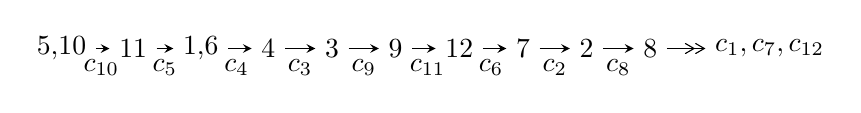
\begin{tikzpicture}[x=23pt, y=7pt]
	% node
	\node (A0) at (-1/8, 0) {5,10};
	\node (A1) at (1, 0) {11};
	\node (A2) at (33/16, 0) {1,6};
	\node (A3) at (25/8, 0) {4};
	\node (A4) at (33/8, 0) {3};
	\node (A5) at (41/8, 0) {9};
	\node (A6) at (49/8, 0) {12};
	\node (A7) at (57/8, 0) {7};
	\node (A8) at (65/8, 0) {2};
	\node (A9) at (73/8, 0) {8};
	\node (C1) at (1/2, -1) {$c_{10}$};
	\node (C2) at (3/2, -1) {$c_{5}$};
	\node (C3) at (21/8, -1) {$c_{4}$};
	\node (C4) at (29/8, -1) {$c_{3}$};
	\node (C5) at (37/8, -1) {$c_{9}$};
	\node (C6) at (45/8, -1) {$c_{11}$};
	\node (C7) at (53/8, -1) {$c_{6}$};
	\node (C8) at (61/8, -1) {$c_{2}$};
	\node (C9) at (69/8, -1) {$c_{8}$};
	\node (A10) at (11, 0) {$c_{1},c_{7},c_{12}$};

	% edge
	\draw[->,>=stealth]	
	(A0) edge (A1) (A1) edge (A2) (A2) edge (A3) (A3) edge (A4) (A4) edge (A5) (A5) edge (A6) (A6) edge (A7) (A7) edge (A8) (A8) edge (A9) ;
	\draw[->>,>={angle 60}]	
	(A9) edge (A10);
\end{tikzpicture} \\ 

\end{tabular} \\

\footnotetext{
The image of knot diagram is generated by the software ``\textbf{Draw programme}" developed by Andrew Bartholomew(\url{http://www.layer8.co.uk/maths/draw/index.htm\#Running-draw}), where we modified some parts for our purpose(\url{https://github.com/CATsTAILs/LinksPainter}).
}\phantom \\ \newline 
\centering \textbf{Ideals for irreducible components\footnotemark of $X_{\text{par}}$} 
 
\begin{align*}
I^u_{1}&=\langle 
2.78909\times10^{906} u^{150}+1.77978\times10^{907} u^{149}+\cdots+6.79585\times10^{909} b+3.55880\times10^{912},\\
\phantom{I^u_{1}}&\phantom{= \langle  }-2.72985\times10^{912} u^{150}-1.18971\times10^{913} u^{149}+\cdots+3.64126\times10^{915} a-1.56273\times10^{918},\\
\phantom{I^u_{1}}&\phantom{= \langle  }u^{151}+3 u^{150}+\cdots-129350 u-535807\rangle \\
I^u_{2}&=\langle 
1.73301\times10^{80} u^{53}-1.72167\times10^{80} u^{52}+\cdots+7.66015\times10^{80} b+3.65973\times10^{81},\\
\phantom{I^u_{2}}&\phantom{= \langle  }4.63544\times10^{81} u^{53}-1.34440\times10^{82} u^{52}+\cdots+8.42616\times10^{81} a+9.73365\times10^{82},\;u^{54}-2 u^{53}+\cdots-43 u+11\rangle \\
I^u_{3}&=\langle 
-282584245189 u^{23}-141467030199 u^{22}+\cdots+3582237958296 b+1522929087540,\\
\phantom{I^u_{3}}&\phantom{= \langle  }-1250731616591 u^{23}-362681281151 u^{22}+\cdots+3582237958296 a+7441470529330,\\
\phantom{I^u_{3}}&\phantom{= \langle  }u^{24}-6 u^{22}+\cdots-11 u+4\rangle \\
\\
\end{align*}
\raggedright * 3 irreducible components of $\dim_{\mathbb{C}}=0$, with total 229 representations.\\
\footnotetext{All coefficients of polynomials are rational numbers. But the coefficients are sometimes approximated in decimal forms when there is not enough margin.}
\newpage
\renewcommand{\arraystretch}{1}
\centering \section*{I. $I^u_{1}= \langle 2.79\times10^{906} u^{150}+1.78\times10^{907} u^{149}+\cdots+6.80\times10^{909} b+3.56\times10^{912},\;-2.73\times10^{912} u^{150}-1.19\times10^{913} u^{149}+\cdots+3.64\times10^{915} a-1.56\times10^{918},\;u^{151}+3 u^{150}+\cdots-129350 u-535807 \rangle$}
\flushleft \textbf{(i) Arc colorings}\\
\begin{tabular}{m{7pt} m{180pt} m{7pt} m{180pt} }
\flushright $a_{5}=$&$\begin{pmatrix}0\\u\end{pmatrix}$ \\
\flushright $a_{10}=$&$\begin{pmatrix}1\\0\end{pmatrix}$ \\
\flushright $a_{11}=$&$\begin{pmatrix}1\\u^2\end{pmatrix}$ \\
\flushright $a_{1}=$&$\begin{pmatrix}0.000749699 u^{150}+0.00326730 u^{149}+\cdots+363.834 u+429.173\\-0.000410410 u^{150}-0.00261892 u^{149}+\cdots-257.671 u-523.672\end{pmatrix}$ \\
\flushright $a_{6}=$&$\begin{pmatrix}- u\\- u^3+u\end{pmatrix}$ \\
\flushright $a_{4}=$&$\begin{pmatrix}-0.000150529 u^{150}-0.000418998 u^{149}+\cdots-47.7340 u+0.0445641\\0.000645914 u^{150}+0.00293879 u^{149}+\cdots+332.117 u+373.399\end{pmatrix}$ \\
\flushright $a_{3}=$&$\begin{pmatrix}0.000495385 u^{150}+0.00251979 u^{149}+\cdots+284.383 u+373.444\\0.000645914 u^{150}+0.00293879 u^{149}+\cdots+332.117 u+373.399\end{pmatrix}$ \\
\flushright $a_{9}=$&$\begin{pmatrix}-0.000269832 u^{150}-0.00118694 u^{149}+\cdots-143.133 u-102.321\\-0.000513616 u^{150}-0.00166823 u^{149}+\cdots-213.719 u-8.85896\end{pmatrix}$ \\
\flushright $a_{12}=$&$\begin{pmatrix}-0.000393228 u^{150}-0.00161135 u^{149}+\cdots-206.157 u-152.825\\-0.000370259 u^{150}-0.00151256 u^{149}+\cdots-145.856 u-181.818\end{pmatrix}$ \\
\flushright $a_{7}=$&$\begin{pmatrix}-0.00100894 u^{150}-0.00351848 u^{149}+\cdots-414.637 u-216.564\\-0.000110272 u^{150}-0.0000858943 u^{149}+\cdots+7.81534 u+60.3391\end{pmatrix}$ \\
\flushright $a_{2}=$&$\begin{pmatrix}-0.000238467 u^{150}-0.00104981 u^{149}+\cdots-120.209 u-81.4658\\0.000692938 u^{150}+0.00243784 u^{149}+\cdots+299.809 u+124.677\end{pmatrix}$ \\
\flushright $a_{8}=$&$\begin{pmatrix}0.000237567 u^{150}+0.000270994 u^{149}+\cdots+60.1651 u-170.428\\-0.000358262 u^{150}-0.00110698 u^{149}+\cdots-153.461 u+24.8154\end{pmatrix}$\\&\end{tabular}
\flushleft \textbf{(ii) Obstruction class $= -1$}\\~\\
\flushleft \textbf{(iii) Cusp Shapes $= 0.00312249 u^{150}+0.0113018 u^{149}+\cdots+1116.10 u+438.520$}\\~\\
\newpage\renewcommand{\arraystretch}{1}
\flushleft \textbf{(iv) u-Polynomials at the component}\newline \\
\begin{tabular}{m{50pt}|m{274pt}}
Crossings & \hspace{64pt}u-Polynomials at each crossing \\
\hline $$\begin{aligned}c_{1},c_{4}\end{aligned}$$&$\begin{aligned}
&u^{151}-6 u^{150}+\cdots+570 u+89
\end{aligned}$\\
\hline $$\begin{aligned}c_{2},c_{7}\end{aligned}$$&$\begin{aligned}
&u^{151}+u^{150}+\cdots-1422 u+995
\end{aligned}$\\
\hline $$\begin{aligned}c_{3},c_{9}\end{aligned}$$&$\begin{aligned}
&u^{151}+25 u^{150}+\cdots+809488384 u+28909568
\end{aligned}$\\
\hline $$\begin{aligned}c_{5},c_{10}\end{aligned}$$&$\begin{aligned}
&u^{151}-3 u^{150}+\cdots-129350 u+535807
\end{aligned}$\\
\hline $$\begin{aligned}c_{6}\end{aligned}$$&$\begin{aligned}
&u^{151}+u^{150}+\cdots+13 u+1
\end{aligned}$\\
\hline $$\begin{aligned}c_{8}\end{aligned}$$&$\begin{aligned}
&u^{151}+29 u^{150}+\cdots-1060088 u-59168
\end{aligned}$\\
\hline $$\begin{aligned}c_{11}\end{aligned}$$&$\begin{aligned}
&u^{151}-11 u^{150}+\cdots+13999 u-2101
\end{aligned}$\\
\hline $$\begin{aligned}c_{12}\end{aligned}$$&$\begin{aligned}
&u^{151}-5 u^{150}+\cdots+5134178638 u+454373173
\end{aligned}$\\
\hline
\end{tabular}\\~\\
\newpage\renewcommand{\arraystretch}{1}
\flushleft \textbf{(v) Riley Polynomials at the component}\newline \\
\begin{tabular}{m{50pt}|m{274pt}}
Crossings & \hspace{64pt}Riley Polynomials at each crossing \\
\hline $$\begin{aligned}c_{1},c_{4}\end{aligned}$$&$\begin{aligned}
&y^{151}+70 y^{150}+\cdots+148680 y-7921
\end{aligned}$\\
\hline $$\begin{aligned}c_{2},c_{7}\end{aligned}$$&$\begin{aligned}
&y^{151}+109 y^{150}+\cdots-58402276 y-990025
\end{aligned}$\\
\hline $$\begin{aligned}c_{3},c_{9}\end{aligned}$$&$\begin{aligned}
&y^{151}-79 y^{150}+\cdots+3044650659086336 y-835763121946624
\end{aligned}$\\
\hline $$\begin{aligned}c_{5},c_{10}\end{aligned}$$&$\begin{aligned}
&y^{151}-131 y^{150}+\cdots+3528966668166 y-287089141249
\end{aligned}$\\
\hline $$\begin{aligned}c_{6}\end{aligned}$$&$\begin{aligned}
&y^{151}-9 y^{150}+\cdots+91 y-1
\end{aligned}$\\
\hline $$\begin{aligned}c_{8}\end{aligned}$$&$\begin{aligned}
&y^{151}- y^{150}+\cdots-239762712768 y-3500852224
\end{aligned}$\\
\hline $$\begin{aligned}c_{11}\end{aligned}$$&$\begin{aligned}
&y^{151}-49 y^{150}+\cdots+489292611 y-4414201
\end{aligned}$\\
\hline $$\begin{aligned}c_{12}\end{aligned}$$&$\begin{aligned}
&y^{151}+11 y^{150}+\cdots-6.12\times10^{18} y-2.06\times10^{17}
\end{aligned}$\\
\hline
\end{tabular}\\~\\
\newpage\flushleft \textbf{(vi) Complex Volumes and Cusp Shapes}
$$\begin{array}{c|c|c}  
\text{Solutions to }I^u_{1}& \I (\text{vol} + \sqrt{-1}CS) & \text{Cusp shape}\\
 \hline 
\begin{aligned}
u &= -0.989621 + 0.201988 I \\
a &= -1.330770 - 0.209572 I \\
b &= \phantom{-}1.031990 - 0.191384 I\end{aligned}
 & -5.97670 + 0.32378 I & \phantom{-0.000000 } 0 \\ \hline\begin{aligned}
u &= -0.989621 - 0.201988 I \\
a &= -1.330770 + 0.209572 I \\
b &= \phantom{-}1.031990 + 0.191384 I\end{aligned}
 & -5.97670 - 0.32378 I & \phantom{-0.000000 } 0 \\ \hline\begin{aligned}
u &= \phantom{-}0.195647 + 0.992750 I \\
a &= \phantom{-}0.101560 + 0.965208 I \\
b &= -1.021620 + 0.241159 I\end{aligned}
 & -4.65085 - 8.19139 I & \phantom{-0.000000 } 0 \\ \hline\begin{aligned}
u &= \phantom{-}0.195647 - 0.992750 I \\
a &= \phantom{-}0.101560 - 0.965208 I \\
b &= -1.021620 - 0.241159 I\end{aligned}
 & -4.65085 + 8.19139 I & \phantom{-0.000000 } 0 \\ \hline\begin{aligned}
u &= -1.029590 + 0.146232 I \\
a &= \phantom{-}0.337774 + 0.748832 I \\
b &= -1.057260 - 0.016984 I\end{aligned}
 & -0.64871 + 4.01069 I & \phantom{-0.000000 } 0 \\ \hline\begin{aligned}
u &= -1.029590 - 0.146232 I \\
a &= \phantom{-}0.337774 - 0.748832 I \\
b &= -1.057260 + 0.016984 I\end{aligned}
 & -0.64871 - 4.01069 I & \phantom{-0.000000 } 0 \\ \hline\begin{aligned}
u &= \phantom{-}0.924459 + 0.487330 I \\
a &= \phantom{-}0.153325 + 0.004777 I \\
b &= -2.63013 + 1.23160 I\end{aligned}
 & -5.67979 - 7.53610 I & \phantom{-0.000000 } 0 \\ \hline\begin{aligned}
u &= \phantom{-}0.924459 - 0.487330 I \\
a &= \phantom{-}0.153325 - 0.004777 I \\
b &= -2.63013 - 1.23160 I\end{aligned}
 & -5.67979 + 7.53610 I & \phantom{-0.000000 } 0 \\ \hline\begin{aligned}
u &= -0.842144 + 0.619436 I \\
a &= -0.603416 + 0.781620 I \\
b &= \phantom{-}1.18333 + 0.95315 I\end{aligned}
 & \phantom{-}3.29033 + 4.04562 I & \phantom{-0.000000 } 0 \\ \hline\begin{aligned}
u &= -0.842144 - 0.619436 I \\
a &= -0.603416 - 0.781620 I \\
b &= \phantom{-}1.18333 - 0.95315 I\end{aligned}
 & \phantom{-}3.29033 - 4.04562 I & \phantom{-0.000000 } 0\\
 \hline 
 \end{array}$$\newpage$$\begin{array}{c|c|c}  
\text{Solutions to }I^u_{1}& \I (\text{vol} + \sqrt{-1}CS) & \text{Cusp shape}\\
 \hline 
\begin{aligned}
u &= -0.932288 + 0.136389 I \\
a &= \phantom{-}0.095187 - 1.404090 I \\
b &= \phantom{-}0.276146 - 1.320560 I\end{aligned}
 & -0.54133 - 3.45770 I & \phantom{-0.000000 } 0 \\ \hline\begin{aligned}
u &= -0.932288 - 0.136389 I \\
a &= \phantom{-}0.095187 + 1.404090 I \\
b &= \phantom{-}0.276146 + 1.320560 I\end{aligned}
 & -0.54133 + 3.45770 I & \phantom{-0.000000 } 0 \\ \hline\begin{aligned}
u &= -0.785433 + 0.512996 I \\
a &= \phantom{-}0.669447 - 0.703718 I \\
b &= -1.53714 - 0.24161 I\end{aligned}
 & \phantom{-}3.43539 + 0.47178 I & \phantom{-0.000000 } 0 \\ \hline\begin{aligned}
u &= -0.785433 - 0.512996 I \\
a &= \phantom{-}0.669447 + 0.703718 I \\
b &= -1.53714 + 0.24161 I\end{aligned}
 & \phantom{-}3.43539 - 0.47178 I & \phantom{-0.000000 } 0 \\ \hline\begin{aligned}
u &= -0.040993 + 0.918125 I \\
a &= -1.155170 + 0.309329 I \\
b &= \phantom{-}1.252510 + 0.591347 I\end{aligned}
 & \phantom{-}4.02575 - 3.19914 I & \phantom{-0.000000 } 0 \\ \hline\begin{aligned}
u &= -0.040993 - 0.918125 I \\
a &= -1.155170 - 0.309329 I \\
b &= \phantom{-}1.252510 - 0.591347 I\end{aligned}
 & \phantom{-}4.02575 + 3.19914 I & \phantom{-0.000000 } 0 \\ \hline\begin{aligned}
u &= -0.014299 + 0.917280 I \\
a &= \phantom{-}1.270090 - 0.264676 I \\
b &= -1.45701 + 0.52769 I\end{aligned}
 & \phantom{-}2.48346 - 2.86698 I & \phantom{-0.000000 } 0 \\ \hline\begin{aligned}
u &= -0.014299 - 0.917280 I \\
a &= \phantom{-}1.270090 + 0.264676 I \\
b &= -1.45701 - 0.52769 I\end{aligned}
 & \phantom{-}2.48346 + 2.86698 I & \phantom{-0.000000 } 0 \\ \hline\begin{aligned}
u &= \phantom{-}1.086560 + 0.180897 I \\
a &= \phantom{-}0.738300 + 0.773623 I \\
b &= -2.00520 + 1.01112 I\end{aligned}
 & -2.19680 - 2.99995 I & \phantom{-0.000000 } 0 \\ \hline\begin{aligned}
u &= \phantom{-}1.086560 - 0.180897 I \\
a &= \phantom{-}0.738300 - 0.773623 I \\
b &= -2.00520 - 1.01112 I\end{aligned}
 & -2.19680 + 2.99995 I & \phantom{-0.000000 } 0\\
 \hline 
 \end{array}$$\newpage$$\begin{array}{c|c|c}  
\text{Solutions to }I^u_{1}& \I (\text{vol} + \sqrt{-1}CS) & \text{Cusp shape}\\
 \hline 
\begin{aligned}
u &= \phantom{-}0.608640 + 0.648787 I \\
a &= \phantom{-}1.235550 + 0.508695 I \\
b &= -0.797078 - 0.409202 I\end{aligned}
 & \phantom{-}1.65331 + 0.22737 I & \phantom{-0.000000 } 0 \\ \hline\begin{aligned}
u &= \phantom{-}0.608640 - 0.648787 I \\
a &= \phantom{-}1.235550 - 0.508695 I \\
b &= -0.797078 + 0.409202 I\end{aligned}
 & \phantom{-}1.65331 - 0.22737 I & \phantom{-0.000000 } 0 \\ \hline\begin{aligned}
u &= \phantom{-}1.131570 + 0.079430 I \\
a &= \phantom{-}0.557842 + 0.718049 I \\
b &= -2.53566 - 0.62292 I\end{aligned}
 & -2.15261 - 2.28421 I & \phantom{-0.000000 } 0 \\ \hline\begin{aligned}
u &= \phantom{-}1.131570 - 0.079430 I \\
a &= \phantom{-}0.557842 - 0.718049 I \\
b &= -2.53566 + 0.62292 I\end{aligned}
 & -2.15261 + 2.28421 I & \phantom{-0.000000 } 0 \\ \hline\begin{aligned}
u &= -1.086910 + 0.325244 I \\
a &= -0.68020 + 1.38185 I \\
b &= \phantom{-}0.555995 + 1.041930 I\end{aligned}
 & \phantom{-}0.11559 + 8.78908 I & \phantom{-0.000000 } 0 \\ \hline\begin{aligned}
u &= -1.086910 - 0.325244 I \\
a &= -0.68020 - 1.38185 I \\
b &= \phantom{-}0.555995 - 1.041930 I\end{aligned}
 & \phantom{-}0.11559 - 8.78908 I & \phantom{-0.000000 } 0 \\ \hline\begin{aligned}
u &= -1.033810 + 0.478244 I \\
a &= \phantom{-}0.934375 - 0.280354 I \\
b &= -1.74148 - 0.45747 I\end{aligned}
 & -1.16547 + 7.92072 I & \phantom{-0.000000 } 0 \\ \hline\begin{aligned}
u &= -1.033810 - 0.478244 I \\
a &= \phantom{-}0.934375 + 0.280354 I \\
b &= -1.74148 + 0.45747 I\end{aligned}
 & -1.16547 - 7.92072 I & \phantom{-0.000000 } 0 \\ \hline\begin{aligned}
u &= -0.239480 + 0.797698 I \\
a &= -1.66465 - 0.06518 I \\
b &= \phantom{-}1.165070 - 0.290693 I\end{aligned}
 & \phantom{-}1.84287 + 8.78656 I & \phantom{-0.000000 } 0 \\ \hline\begin{aligned}
u &= -0.239480 - 0.797698 I \\
a &= -1.66465 + 0.06518 I \\
b &= \phantom{-}1.165070 + 0.290693 I\end{aligned}
 & \phantom{-}1.84287 - 8.78656 I & \phantom{-0.000000 } 0\\
 \hline 
 \end{array}$$\newpage$$\begin{array}{c|c|c}  
\text{Solutions to }I^u_{1}& \I (\text{vol} + \sqrt{-1}CS) & \text{Cusp shape}\\
 \hline 
\begin{aligned}
u &= -0.695070 + 0.939006 I \\
a &= \phantom{-}1.090170 - 0.024159 I \\
b &= -1.56812 - 0.52401 I\end{aligned}
 & \phantom{-}0.79650 + 2.81303 I & \phantom{-0.000000 } 0 \\ \hline\begin{aligned}
u &= -0.695070 - 0.939006 I \\
a &= \phantom{-}1.090170 + 0.024159 I \\
b &= -1.56812 + 0.52401 I\end{aligned}
 & \phantom{-}0.79650 - 2.81303 I & \phantom{-0.000000 } 0 \\ \hline\begin{aligned}
u &= \phantom{-}0.419965 + 1.101130 I \\
a &= \phantom{-}1.234950 + 0.047860 I \\
b &= -1.47189 + 0.37047 I\end{aligned}
 & \phantom{-}1.81514 - 1.66518 I & \phantom{-0.000000 } 0 \\ \hline\begin{aligned}
u &= \phantom{-}0.419965 - 1.101130 I \\
a &= \phantom{-}1.234950 - 0.047860 I \\
b &= -1.47189 - 0.37047 I\end{aligned}
 & \phantom{-}1.81514 + 1.66518 I & \phantom{-0.000000 } 0 \\ \hline\begin{aligned}
u &= \phantom{-}1.186160 + 0.018466 I \\
a &= -0.336979 - 0.813641 I \\
b &= \phantom{-}1.049530 - 0.539248 I\end{aligned}
 & -1.116100 - 0.815767 I & \phantom{-0.000000 } 0 \\ \hline\begin{aligned}
u &= \phantom{-}1.186160 - 0.018466 I \\
a &= -0.336979 + 0.813641 I \\
b &= \phantom{-}1.049530 + 0.539248 I\end{aligned}
 & -1.116100 + 0.815767 I & \phantom{-0.000000 } 0 \\ \hline\begin{aligned}
u &= \phantom{-}1.185190 + 0.081323 I \\
a &= -1.178090 + 0.567113 I \\
b &= \phantom{-}0.0118928 - 0.1371670 I\end{aligned}
 & -9.18886 - 1.94213 I & \phantom{-0.000000 } 0 \\ \hline\begin{aligned}
u &= \phantom{-}1.185190 - 0.081323 I \\
a &= -1.178090 - 0.567113 I \\
b &= \phantom{-}0.0118928 + 0.1371670 I\end{aligned}
 & -9.18886 + 1.94213 I & \phantom{-0.000000 } 0 \\ \hline\begin{aligned}
u &= \phantom{-}1.199840 + 0.016721 I \\
a &= \phantom{-}0.569267 + 0.694885 I \\
b &= -0.975285 - 0.617361 I\end{aligned}
 & -2.62660 - 2.23776 I & \phantom{-0.000000 } 0 \\ \hline\begin{aligned}
u &= \phantom{-}1.199840 - 0.016721 I \\
a &= \phantom{-}0.569267 - 0.694885 I \\
b &= -0.975285 + 0.617361 I\end{aligned}
 & -2.62660 + 2.23776 I & \phantom{-0.000000 } 0\\
 \hline 
 \end{array}$$\newpage$$\begin{array}{c|c|c}  
\text{Solutions to }I^u_{1}& \I (\text{vol} + \sqrt{-1}CS) & \text{Cusp shape}\\
 \hline 
\begin{aligned}
u &= -0.628319 + 1.025400 I \\
a &= \phantom{-}1.077340 - 0.573236 I \\
b &= -1.214200 + 0.231562 I\end{aligned}
 & \phantom{-}1.58459 - 4.07369 I & \phantom{-0.000000 } 0 \\ \hline\begin{aligned}
u &= -0.628319 - 1.025400 I \\
a &= \phantom{-}1.077340 + 0.573236 I \\
b &= -1.214200 - 0.231562 I\end{aligned}
 & \phantom{-}1.58459 + 4.07369 I & \phantom{-0.000000 } 0 \\ \hline\begin{aligned}
u &= \phantom{-}1.178530 + 0.265679 I \\
a &= -0.966890 - 0.906870 I \\
b &= \phantom{-}1.26949 - 1.06631 I\end{aligned}
 & -6.64560 - 10.08510 I & \phantom{-0.000000 } 0 \\ \hline\begin{aligned}
u &= \phantom{-}1.178530 - 0.265679 I \\
a &= -0.966890 + 0.906870 I \\
b &= \phantom{-}1.26949 + 1.06631 I\end{aligned}
 & -6.64560 + 10.08510 I & \phantom{-0.000000 } 0 \\ \hline\begin{aligned}
u &= \phantom{-}0.087688 + 0.785135 I \\
a &= \phantom{-}0.101352 - 1.238340 I \\
b &= \phantom{-}0.235453 - 0.079604 I\end{aligned}
 & -2.35988 + 3.71556 I & \phantom{-0.000000 } 0 \\ \hline\begin{aligned}
u &= \phantom{-}0.087688 - 0.785135 I \\
a &= \phantom{-}0.101352 + 1.238340 I \\
b &= \phantom{-}0.235453 + 0.079604 I\end{aligned}
 & -2.35988 - 3.71556 I & \phantom{-0.000000 } 0 \\ \hline\begin{aligned}
u &= -1.210980 + 0.022993 I \\
a &= \phantom{-}0.398547 - 0.779594 I \\
b &= -1.55343 - 2.07829 I\end{aligned}
 & -10.10550 - 1.91827 I & \phantom{-0.000000 } 0 \\ \hline\begin{aligned}
u &= -1.210980 - 0.022993 I \\
a &= \phantom{-}0.398547 + 0.779594 I \\
b &= -1.55343 + 2.07829 I\end{aligned}
 & -10.10550 + 1.91827 I & \phantom{-0.000000 } 0 \\ \hline\begin{aligned}
u &= -1.203270 + 0.220242 I \\
a &= -0.798951 + 0.893305 I \\
b &= \phantom{-}1.23314 + 1.07555 I\end{aligned}
 & -3.55896 + 5.56320 I & \phantom{-0.000000 } 0 \\ \hline\begin{aligned}
u &= -1.203270 - 0.220242 I \\
a &= -0.798951 - 0.893305 I \\
b &= \phantom{-}1.23314 - 1.07555 I\end{aligned}
 & -3.55896 - 5.56320 I & \phantom{-0.000000 } 0\\
 \hline 
 \end{array}$$\newpage$$\begin{array}{c|c|c}  
\text{Solutions to }I^u_{1}& \I (\text{vol} + \sqrt{-1}CS) & \text{Cusp shape}\\
 \hline 
\begin{aligned}
u &= \phantom{-}1.191840 + 0.289597 I \\
a &= -0.313367 - 0.780595 I \\
b &= \phantom{-}1.60916 - 0.38432 I\end{aligned}
 & \phantom{-}0.176558 - 0.397747 I & \phantom{-0.000000 } 0 \\ \hline\begin{aligned}
u &= \phantom{-}1.191840 - 0.289597 I \\
a &= -0.313367 + 0.780595 I \\
b &= \phantom{-}1.60916 + 0.38432 I\end{aligned}
 & \phantom{-}0.176558 + 0.397747 I & \phantom{-0.000000 } 0 \\ \hline\begin{aligned}
u &= -1.180870 + 0.334257 I \\
a &= -0.687722 - 0.516559 I \\
b &= \phantom{-}1.034490 - 0.173996 I\end{aligned}
 & -6.34709 - 0.01164 I & \phantom{-0.000000 } 0 \\ \hline\begin{aligned}
u &= -1.180870 - 0.334257 I \\
a &= -0.687722 + 0.516559 I \\
b &= \phantom{-}1.034490 + 0.173996 I\end{aligned}
 & -6.34709 + 0.01164 I & \phantom{-0.000000 } 0 \\ \hline\begin{aligned}
u &= -0.229732 + 0.730854 I \\
a &= -0.91153 + 1.14541 I \\
b &= \phantom{-}1.46688 - 0.17101 I\end{aligned}
 & -2.70877 - 7.53291 I & \phantom{-0.000000 } 0 \\ \hline\begin{aligned}
u &= -0.229732 - 0.730854 I \\
a &= -0.91153 - 1.14541 I \\
b &= \phantom{-}1.46688 + 0.17101 I\end{aligned}
 & -2.70877 + 7.53291 I & \phantom{-0.000000 } 0 \\ \hline\begin{aligned}
u &= \phantom{-}1.186400 + 0.364122 I \\
a &= \phantom{-}0.502048 - 0.437452 I \\
b &= -1.59308 + 0.10936 I\end{aligned}
 & -5.72474 - 7.93365 I & \phantom{-0.000000 } 0 \\ \hline\begin{aligned}
u &= \phantom{-}1.186400 - 0.364122 I \\
a &= \phantom{-}0.502048 + 0.437452 I \\
b &= -1.59308 - 0.10936 I\end{aligned}
 & -5.72474 + 7.93365 I & \phantom{-0.000000 } 0 \\ \hline\begin{aligned}
u &= \phantom{-}1.26871\phantom{ +0.000000I} \\
a &= \phantom{-}0.517408\phantom{ +0.000000I} \\
b &= \phantom{-}0.241829\phantom{ +0.000000I}\end{aligned}
 & -3.38525\phantom{ +0.000000I} & \phantom{-0.000000 } 0 \\ \hline\begin{aligned}
u &= -1.263770 + 0.123102 I \\
a &= -0.393794 + 0.673452 I \\
b &= \phantom{-}2.02171 + 0.17657 I\end{aligned}
 & -0.01782 + 1.69227 I & \phantom{-0.000000 } 0\\
 \hline 
 \end{array}$$\newpage$$\begin{array}{c|c|c}  
\text{Solutions to }I^u_{1}& \I (\text{vol} + \sqrt{-1}CS) & \text{Cusp shape}\\
 \hline 
\begin{aligned}
u &= -1.263770 - 0.123102 I \\
a &= -0.393794 - 0.673452 I \\
b &= \phantom{-}2.02171 - 0.17657 I\end{aligned}
 & -0.01782 - 1.69227 I & \phantom{-0.000000 } 0 \\ \hline\begin{aligned}
u &= \phantom{-}0.103548 + 0.715178 I \\
a &= \phantom{-}0.864427 + 1.076480 I \\
b &= -0.936398 - 0.457335 I\end{aligned}
 & -3.30497 - 2.46768 I & \phantom{-0.000000 } 0 \\ \hline\begin{aligned}
u &= \phantom{-}0.103548 - 0.715178 I \\
a &= \phantom{-}0.864427 - 1.076480 I \\
b &= -0.936398 + 0.457335 I\end{aligned}
 & -3.30497 + 2.46768 I & \phantom{-0.000000 } 0 \\ \hline\begin{aligned}
u &= -1.227180 + 0.387109 I \\
a &= \phantom{-}0.779630 - 0.661051 I \\
b &= -1.88535 - 1.29000 I\end{aligned}
 & -5.86046 + 11.71370 I & \phantom{-0.000000 } 0 \\ \hline\begin{aligned}
u &= -1.227180 - 0.387109 I \\
a &= \phantom{-}0.779630 + 0.661051 I \\
b &= -1.88535 + 1.29000 I\end{aligned}
 & -5.86046 - 11.71370 I & \phantom{-0.000000 } 0 \\ \hline\begin{aligned}
u &= \phantom{-}0.635202 + 0.316199 I \\
a &= \phantom{-}0.053034 - 1.161830 I \\
b &= \phantom{-}1.233790 - 0.169281 I\end{aligned}
 & -0.915896 + 0.914335 I & \phantom{-0.000000 } 0 \\ \hline\begin{aligned}
u &= \phantom{-}0.635202 - 0.316199 I \\
a &= \phantom{-}0.053034 + 1.161830 I \\
b &= \phantom{-}1.233790 + 0.169281 I\end{aligned}
 & -0.915896 - 0.914335 I & \phantom{-0.000000 } 0 \\ \hline\begin{aligned}
u &= -1.277450 + 0.233343 I \\
a &= \phantom{-}0.625894 + 0.527686 I \\
b &= \phantom{-}0.012172 - 0.347496 I\end{aligned}
 & -7.64715 + 5.75381 I & \phantom{-0.000000 } 0 \\ \hline\begin{aligned}
u &= -1.277450 - 0.233343 I \\
a &= \phantom{-}0.625894 - 0.527686 I \\
b &= \phantom{-}0.012172 + 0.347496 I\end{aligned}
 & -7.64715 - 5.75381 I & \phantom{-0.000000 } 0 \\ \hline\begin{aligned}
u &= \phantom{-}0.666922 + 0.200410 I \\
a &= \phantom{-}0.261037 - 1.159800 I \\
b &= \phantom{-}1.26351 - 0.81653 I\end{aligned}
 & -0.96603 + 1.13617 I & \phantom{-}12.53695 + 0. I\phantom{ +0.000000I}\\
 \hline 
 \end{array}$$\newpage$$\begin{array}{c|c|c}  
\text{Solutions to }I^u_{1}& \I (\text{vol} + \sqrt{-1}CS) & \text{Cusp shape}\\
 \hline 
\begin{aligned}
u &= \phantom{-}0.666922 - 0.200410 I \\
a &= \phantom{-}0.261037 + 1.159800 I \\
b &= \phantom{-}1.26351 + 0.81653 I\end{aligned}
 & -0.96603 - 1.13617 I & \phantom{-}12.53695 + 0. I\phantom{ +0.000000I} \\ \hline\begin{aligned}
u &= \phantom{-}0.137805 + 0.680821 I \\
a &= \phantom{-}1.74045 + 0.11392 I \\
b &= -1.48404 + 0.43443 I\end{aligned}
 & \phantom{-}3.41391 - 3.17991 I & \phantom{-}5.95844 + 8.12878 I \\ \hline\begin{aligned}
u &= \phantom{-}0.137805 - 0.680821 I \\
a &= \phantom{-}1.74045 - 0.11392 I \\
b &= -1.48404 - 0.43443 I\end{aligned}
 & \phantom{-}3.41391 + 3.17991 I & \phantom{-}5.95844 - 8.12878 I \\ \hline\begin{aligned}
u &= \phantom{-}1.116370 + 0.736754 I \\
a &= -0.450058 - 0.847177 I \\
b &= \phantom{-}1.094290 - 0.246895 I\end{aligned}
 & -0.42705 - 4.70858 I & \phantom{-0.000000 } 0 \\ \hline\begin{aligned}
u &= \phantom{-}1.116370 - 0.736754 I \\
a &= -0.450058 + 0.847177 I \\
b &= \phantom{-}1.094290 + 0.246895 I\end{aligned}
 & -0.42705 + 4.70858 I & \phantom{-0.000000 } 0 \\ \hline\begin{aligned}
u &= \phantom{-}1.266710 + 0.463259 I \\
a &= -0.464537 - 0.479341 I \\
b &= \phantom{-}1.44687 - 0.31122 I\end{aligned}
 & -1.58687 - 2.36382 I & \phantom{-0.000000 } 0 \\ \hline\begin{aligned}
u &= \phantom{-}1.266710 - 0.463259 I \\
a &= -0.464537 + 0.479341 I \\
b &= \phantom{-}1.44687 + 0.31122 I\end{aligned}
 & -1.58687 + 2.36382 I & \phantom{-0.000000 } 0 \\ \hline\begin{aligned}
u &= -1.344700 + 0.117596 I \\
a &= -0.881978 + 0.016553 I \\
b &= \phantom{-}0.215971 - 0.056476 I\end{aligned}
 & -6.72520 + 1.37500 I & \phantom{-0.000000 } 0 \\ \hline\begin{aligned}
u &= -1.344700 - 0.117596 I \\
a &= -0.881978 - 0.016553 I \\
b &= \phantom{-}0.215971 + 0.056476 I\end{aligned}
 & -6.72520 - 1.37500 I & \phantom{-0.000000 } 0 \\ \hline\begin{aligned}
u &= \phantom{-}1.348120 + 0.072768 I \\
a &= -0.411708 + 0.644962 I \\
b &= \phantom{-}1.89920 + 1.58101 I\end{aligned}
 & -8.21282 + 4.76264 I & \phantom{-0.000000 } 0\\
 \hline 
 \end{array}$$\newpage$$\begin{array}{c|c|c}  
\text{Solutions to }I^u_{1}& \I (\text{vol} + \sqrt{-1}CS) & \text{Cusp shape}\\
 \hline 
\begin{aligned}
u &= \phantom{-}1.348120 - 0.072768 I \\
a &= -0.411708 - 0.644962 I \\
b &= \phantom{-}1.89920 - 1.58101 I\end{aligned}
 & -8.21282 - 4.76264 I & \phantom{-0.000000 } 0 \\ \hline\begin{aligned}
u &= -1.351950 + 0.017095 I \\
a &= -0.430479 - 0.932062 I \\
b &= \phantom{-}0.839409 - 0.751971 I\end{aligned}
 & -2.00215 - 5.67221 I & \phantom{-0.000000 } 0 \\ \hline\begin{aligned}
u &= -1.351950 - 0.017095 I \\
a &= -0.430479 + 0.932062 I \\
b &= \phantom{-}0.839409 + 0.751971 I\end{aligned}
 & -2.00215 + 5.67221 I & \phantom{-0.000000 } 0 \\ \hline\begin{aligned}
u &= \phantom{-}1.322100 + 0.303321 I \\
a &= -0.605950 - 0.791118 I \\
b &= \phantom{-}1.50324 - 1.59347 I\end{aligned}
 & -4.42620 - 9.52734 I & \phantom{-0.000000 } 0 \\ \hline\begin{aligned}
u &= \phantom{-}1.322100 - 0.303321 I \\
a &= -0.605950 + 0.791118 I \\
b &= \phantom{-}1.50324 + 1.59347 I\end{aligned}
 & -4.42620 + 9.52734 I & \phantom{-0.000000 } 0 \\ \hline\begin{aligned}
u &= -1.340000 + 0.231429 I \\
a &= -0.745977 + 0.744326 I \\
b &= \phantom{-}1.142940 + 0.832721 I\end{aligned}
 & -4.35348 + 5.51402 I & \phantom{-0.000000 } 0 \\ \hline\begin{aligned}
u &= -1.340000 - 0.231429 I \\
a &= -0.745977 - 0.744326 I \\
b &= \phantom{-}1.142940 - 0.832721 I\end{aligned}
 & -4.35348 - 5.51402 I & \phantom{-0.000000 } 0 \\ \hline\begin{aligned}
u &= -1.301210 + 0.454938 I \\
a &= \phantom{-}0.572759 - 0.516468 I \\
b &= -1.72100 - 0.34050 I\end{aligned}
 & \phantom{-}0.02293 + 8.11047 I & \phantom{-0.000000 } 0 \\ \hline\begin{aligned}
u &= -1.301210 - 0.454938 I \\
a &= \phantom{-}0.572759 + 0.516468 I \\
b &= -1.72100 + 0.34050 I\end{aligned}
 & \phantom{-}0.02293 - 8.11047 I & \phantom{-0.000000 } 0 \\ \hline\begin{aligned}
u &= -1.331420 + 0.368886 I \\
a &= -0.666291 + 0.871423 I \\
b &= \phantom{-}1.29321 + 1.21938 I\end{aligned}
 & -1.79274 + 7.42457 I & \phantom{-0.000000 } 0\\
 \hline 
 \end{array}$$\newpage$$\begin{array}{c|c|c}  
\text{Solutions to }I^u_{1}& \I (\text{vol} + \sqrt{-1}CS) & \text{Cusp shape}\\
 \hline 
\begin{aligned}
u &= -1.331420 - 0.368886 I \\
a &= -0.666291 - 0.871423 I \\
b &= \phantom{-}1.29321 - 1.21938 I\end{aligned}
 & -1.79274 - 7.42457 I & \phantom{-0.000000 } 0 \\ \hline\begin{aligned}
u &= \phantom{-}0.026405 + 0.616604 I \\
a &= \phantom{-}1.45663 + 0.62859 I \\
b &= -1.62245 - 0.72311 I\end{aligned}
 & -0.20238 + 6.06846 I & \phantom{-}3.67652 - 7.39581 I \\ \hline\begin{aligned}
u &= \phantom{-}0.026405 - 0.616604 I \\
a &= \phantom{-}1.45663 - 0.62859 I \\
b &= -1.62245 + 0.72311 I\end{aligned}
 & -0.20238 - 6.06846 I & \phantom{-}3.67652 + 7.39581 I \\ \hline\begin{aligned}
u &= -0.517747 + 0.332482 I \\
a &= -0.603630 + 0.433052 I \\
b &= -0.498698 - 0.436422 I\end{aligned}
 & -0.28235 + 4.11135 I & -4.20800 - 7.14416 I \\ \hline\begin{aligned}
u &= -0.517747 - 0.332482 I \\
a &= -0.603630 - 0.433052 I \\
b &= -0.498698 + 0.436422 I\end{aligned}
 & -0.28235 - 4.11135 I & -4.20800 + 7.14416 I \\ \hline\begin{aligned}
u &= \phantom{-}0.352455 + 0.502252 I \\
a &= \phantom{-}0.95196 + 1.92702 I \\
b &= -0.856412 - 0.465099 I\end{aligned}
 & -4.07138 + 7.13413 I & -5.64153 - 7.85475 I \\ \hline\begin{aligned}
u &= \phantom{-}0.352455 - 0.502252 I \\
a &= \phantom{-}0.95196 - 1.92702 I \\
b &= -0.856412 + 0.465099 I\end{aligned}
 & -4.07138 - 7.13413 I & -5.64153 + 7.85475 I \\ \hline\begin{aligned}
u &= \phantom{-}0.561878 + 0.180974 I \\
a &= \phantom{-}0.582727 + 0.163441 I \\
b &= \phantom{-}0.502900 + 0.322357 I\end{aligned}
 & -1.137050 - 0.709680 I & -6.09225 + 1.45743 I \\ \hline\begin{aligned}
u &= \phantom{-}0.561878 - 0.180974 I \\
a &= \phantom{-}0.582727 - 0.163441 I \\
b &= \phantom{-}0.502900 - 0.322357 I\end{aligned}
 & -1.137050 + 0.709680 I & -6.09225 - 1.45743 I \\ \hline\begin{aligned}
u &= -0.240479 + 0.528061 I \\
a &= \phantom{-}0.278878 + 0.438973 I \\
b &= -0.198193 + 0.249502 I\end{aligned}
 & \phantom{-}1.26193 - 0.96699 I & \phantom{-}3.36748 + 0.94788 I\\
 \hline 
 \end{array}$$\newpage$$\begin{array}{c|c|c}  
\text{Solutions to }I^u_{1}& \I (\text{vol} + \sqrt{-1}CS) & \text{Cusp shape}\\
 \hline 
\begin{aligned}
u &= -0.240479 - 0.528061 I \\
a &= \phantom{-}0.278878 - 0.438973 I \\
b &= -0.198193 - 0.249502 I\end{aligned}
 & \phantom{-}1.26193 + 0.96699 I & \phantom{-}3.36748 - 0.94788 I \\ \hline\begin{aligned}
u &= \phantom{-}0.22398 + 1.40552 I \\
a &= -0.882443 + 0.308104 I \\
b &= \phantom{-}1.80574 - 0.35041 I\end{aligned}
 & -2.06865 - 13.83450 I & \phantom{-0.000000 } 0 \\ \hline\begin{aligned}
u &= \phantom{-}0.22398 - 1.40552 I \\
a &= -0.882443 - 0.308104 I \\
b &= \phantom{-}1.80574 + 0.35041 I\end{aligned}
 & -2.06865 + 13.83450 I & \phantom{-0.000000 } 0 \\ \hline\begin{aligned}
u &= \phantom{-}1.42459 + 0.06763 I \\
a &= -0.614236 + 0.328732 I \\
b &= -0.067413 + 0.198167 I\end{aligned}
 & -8.50745 + 4.93640 I & \phantom{-0.000000 } 0 \\ \hline\begin{aligned}
u &= \phantom{-}1.42459 - 0.06763 I \\
a &= -0.614236 - 0.328732 I \\
b &= -0.067413 - 0.198167 I\end{aligned}
 & -8.50745 - 4.93640 I & \phantom{-0.000000 } 0 \\ \hline\begin{aligned}
u &= -1.40351 + 0.37924 I \\
a &= -0.669391 + 0.614115 I \\
b &= \phantom{-}1.42576 + 0.39497 I\end{aligned}
 & -4.26323 + 6.00112 I & \phantom{-0.000000 } 0 \\ \hline\begin{aligned}
u &= -1.40351 - 0.37924 I \\
a &= -0.669391 - 0.614115 I \\
b &= \phantom{-}1.42576 - 0.39497 I\end{aligned}
 & -4.26323 - 6.00112 I & \phantom{-0.000000 } 0 \\ \hline\begin{aligned}
u &= \phantom{-}1.43301 + 0.37070 I \\
a &= \phantom{-}0.587857 + 0.631114 I \\
b &= -1.72880 + 0.15451 I\end{aligned}
 & -3.51012 - 13.13470 I & \phantom{-0.000000 } 0 \\ \hline\begin{aligned}
u &= \phantom{-}1.43301 - 0.37070 I \\
a &= \phantom{-}0.587857 - 0.631114 I \\
b &= -1.72880 - 0.15451 I\end{aligned}
 & -3.51012 + 13.13470 I & \phantom{-0.000000 } 0 \\ \hline\begin{aligned}
u &= \phantom{-}1.44117 + 0.35913 I \\
a &= \phantom{-}0.614950 - 0.387708 I \\
b &= -0.0649504 - 0.0856047 I\end{aligned}
 & -6.48069 - 7.66786 I & \phantom{-0.000000 } 0\\
 \hline 
 \end{array}$$\newpage$$\begin{array}{c|c|c}  
\text{Solutions to }I^u_{1}& \I (\text{vol} + \sqrt{-1}CS) & \text{Cusp shape}\\
 \hline 
\begin{aligned}
u &= \phantom{-}1.44117 - 0.35913 I \\
a &= \phantom{-}0.614950 + 0.387708 I \\
b &= -0.0649504 + 0.0856047 I\end{aligned}
 & -6.48069 + 7.66786 I & \phantom{-0.000000 } 0 \\ \hline\begin{aligned}
u &= -1.42027 + 0.45853 I \\
a &= \phantom{-}0.673911 + 0.617842 I \\
b &= -0.0913554 - 0.0274073 I\end{aligned}
 & -9.7118 + 13.4451 I & \phantom{-0.000000 } 0 \\ \hline\begin{aligned}
u &= -1.42027 - 0.45853 I \\
a &= \phantom{-}0.673911 - 0.617842 I \\
b &= -0.0913554 + 0.0274073 I\end{aligned}
 & -9.7118 - 13.4451 I & \phantom{-0.000000 } 0 \\ \hline\begin{aligned}
u &= -1.40105 + 0.53521 I \\
a &= \phantom{-}0.569791 - 0.489838 I \\
b &= -1.78754 - 1.86093 I\end{aligned}
 & -10.62830 + 7.42736 I & \phantom{-0.000000 } 0 \\ \hline\begin{aligned}
u &= -1.40105 - 0.53521 I \\
a &= \phantom{-}0.569791 + 0.489838 I \\
b &= -1.78754 + 1.86093 I\end{aligned}
 & -10.62830 - 7.42736 I & \phantom{-0.000000 } 0 \\ \hline\begin{aligned}
u &= \phantom{-}1.35137 + 0.65290 I \\
a &= -0.528261 + 0.791645 I \\
b &= -0.021432 + 0.178966 I\end{aligned}
 & -10.06200 - 3.93216 I & \phantom{-0.000000 } 0 \\ \hline\begin{aligned}
u &= \phantom{-}1.35137 - 0.65290 I \\
a &= -0.528261 - 0.791645 I \\
b &= -0.021432 - 0.178966 I\end{aligned}
 & -10.06200 + 3.93216 I & \phantom{-0.000000 } 0 \\ \hline\begin{aligned}
u &= -0.20719 + 1.48996 I \\
a &= -0.710545 - 0.222258 I \\
b &= \phantom{-}2.00454 + 0.39262 I\end{aligned}
 & \phantom{-}1.42160 + 6.81005 I & \phantom{-0.000000 } 0 \\ \hline\begin{aligned}
u &= -0.20719 - 1.48996 I \\
a &= -0.710545 + 0.222258 I \\
b &= \phantom{-}2.00454 - 0.39262 I\end{aligned}
 & \phantom{-}1.42160 - 6.81005 I & \phantom{-0.000000 } 0 \\ \hline\begin{aligned}
u &= \phantom{-}0.021373 + 0.487123 I \\
a &= -0.03131 + 1.52211 I \\
b &= \phantom{-}1.47558 + 0.53439 I\end{aligned}
 & -6.84707 - 1.57322 I & -11.20662 + 3.99424 I\\
 \hline 
 \end{array}$$\newpage$$\begin{array}{c|c|c}  
\text{Solutions to }I^u_{1}& \I (\text{vol} + \sqrt{-1}CS) & \text{Cusp shape}\\
 \hline 
\begin{aligned}
u &= \phantom{-}0.021373 - 0.487123 I \\
a &= -0.03131 - 1.52211 I \\
b &= \phantom{-}1.47558 - 0.53439 I\end{aligned}
 & -6.84707 + 1.57322 I & -11.20662 - 3.99424 I \\ \hline\begin{aligned}
u &= \phantom{-}0.423933 + 0.232833 I \\
a &= \phantom{-}1.197130 + 0.084477 I \\
b &= \phantom{-}0.221878 + 0.656554 I\end{aligned}
 & -1.24682 - 1.15343 I & -2.63294 + 5.49737 I \\ \hline\begin{aligned}
u &= \phantom{-}0.423933 - 0.232833 I \\
a &= \phantom{-}1.197130 - 0.084477 I \\
b &= \phantom{-}0.221878 - 0.656554 I\end{aligned}
 & -1.24682 + 1.15343 I & -2.63294 - 5.49737 I \\ \hline\begin{aligned}
u &= -1.52130 + 0.01187 I \\
a &= \phantom{-}0.262601 + 0.518135 I \\
b &= -0.081759 - 0.535539 I\end{aligned}
 & -10.73120 - 5.55715 I & \phantom{-0.000000 } 0 \\ \hline\begin{aligned}
u &= -1.52130 - 0.01187 I \\
a &= \phantom{-}0.262601 - 0.518135 I \\
b &= -0.081759 + 0.535539 I\end{aligned}
 & -10.73120 + 5.55715 I & \phantom{-0.000000 } 0 \\ \hline\begin{aligned}
u &= -0.452519 + 0.091194 I \\
a &= -0.89989 + 1.51014 I \\
b &= -0.666509 - 0.341622 I\end{aligned}
 & -0.23151 + 4.11735 I & -4.65728 - 6.18703 I \\ \hline\begin{aligned}
u &= -0.452519 - 0.091194 I \\
a &= -0.89989 - 1.51014 I \\
b &= -0.666509 + 0.341622 I\end{aligned}
 & -0.23151 - 4.11735 I & -4.65728 + 6.18703 I \\ \hline\begin{aligned}
u &= \phantom{-}0.49169 + 1.46138 I \\
a &= \phantom{-}0.544485 + 0.566434 I \\
b &= -1.49887 + 0.03397 I\end{aligned}
 & -4.49884 + 3.03697 I & \phantom{-0.000000 } 0 \\ \hline\begin{aligned}
u &= \phantom{-}0.49169 - 1.46138 I \\
a &= \phantom{-}0.544485 - 0.566434 I \\
b &= -1.49887 - 0.03397 I\end{aligned}
 & -4.49884 - 3.03697 I & \phantom{-0.000000 } 0 \\ \hline\begin{aligned}
u &= \phantom{-}1.56061 + 0.10706 I \\
a &= -0.116307 + 0.246242 I \\
b &= \phantom{-}0.016091 - 0.478918 I\end{aligned}
 & -7.80280 - 5.42649 I & \phantom{-0.000000 } 0\\
 \hline 
 \end{array}$$\newpage$$\begin{array}{c|c|c}  
\text{Solutions to }I^u_{1}& \I (\text{vol} + \sqrt{-1}CS) & \text{Cusp shape}\\
 \hline 
\begin{aligned}
u &= \phantom{-}1.56061 - 0.10706 I \\
a &= -0.116307 - 0.246242 I \\
b &= \phantom{-}0.016091 + 0.478918 I\end{aligned}
 & -7.80280 + 5.42649 I & \phantom{-0.000000 } 0 \\ \hline\begin{aligned}
u &= \phantom{-}1.49158 + 0.57501 I \\
a &= \phantom{-}0.659165 + 0.548921 I \\
b &= -1.71740 + 1.40334 I\end{aligned}
 & -3.8756 - 13.7118 I & \phantom{-0.000000 } 0 \\ \hline\begin{aligned}
u &= \phantom{-}1.49158 - 0.57501 I \\
a &= \phantom{-}0.659165 - 0.548921 I \\
b &= -1.71740 - 1.40334 I\end{aligned}
 & -3.8756 + 13.7118 I & \phantom{-0.000000 } 0 \\ \hline\begin{aligned}
u &= -0.221972 + 0.322484 I \\
a &= \phantom{-}1.93378 - 1.50615 I \\
b &= -1.41122 - 0.44461 I\end{aligned}
 & \phantom{-}3.31418 - 0.17339 I & \phantom{-}5.19920 - 0.83619 I \\ \hline\begin{aligned}
u &= -0.221972 - 0.322484 I \\
a &= \phantom{-}1.93378 + 1.50615 I \\
b &= -1.41122 + 0.44461 I\end{aligned}
 & \phantom{-}3.31418 + 0.17339 I & \phantom{-}5.19920 + 0.83619 I \\ \hline\begin{aligned}
u &= -1.51370 + 0.57178 I \\
a &= \phantom{-}0.731304 - 0.540077 I \\
b &= -1.81834 - 1.21173 I\end{aligned}
 & -7.4956 + 20.6334 I & \phantom{-0.000000 } 0 \\ \hline\begin{aligned}
u &= -1.51370 - 0.57178 I \\
a &= \phantom{-}0.731304 + 0.540077 I \\
b &= -1.81834 + 1.21173 I\end{aligned}
 & -7.4956 - 20.6334 I & \phantom{-0.000000 } 0 \\ \hline\begin{aligned}
u &= -1.59809 + 0.35010 I \\
a &= \phantom{-}0.244082 + 0.485375 I \\
b &= \phantom{-}0.207672 + 0.051096 I\end{aligned}
 & -11.60660 + 3.02641 I & \phantom{-0.000000 } 0 \\ \hline\begin{aligned}
u &= -1.59809 - 0.35010 I \\
a &= \phantom{-}0.244082 - 0.485375 I \\
b &= \phantom{-}0.207672 - 0.051096 I\end{aligned}
 & -11.60660 - 3.02641 I & \phantom{-0.000000 } 0 \\ \hline\begin{aligned}
u &= \phantom{-}1.66903 + 0.00947 I \\
a &= -0.372767 + 0.521914 I \\
b &= \phantom{-}0.554735 - 0.138348 I\end{aligned}
 & -8.12071 + 0.05756 I & \phantom{-0.000000 } 0\\
 \hline 
 \end{array}$$\newpage$$\begin{array}{c|c|c}  
\text{Solutions to }I^u_{1}& \I (\text{vol} + \sqrt{-1}CS) & \text{Cusp shape}\\
 \hline 
\begin{aligned}
u &= \phantom{-}1.66903 - 0.00947 I \\
a &= -0.372767 - 0.521914 I \\
b &= \phantom{-}0.554735 + 0.138348 I\end{aligned}
 & -8.12071 - 0.05756 I & \phantom{-0.000000 } 0 \\ \hline\begin{aligned}
u &= \phantom{-}0.146949 + 0.294093 I \\
a &= \phantom{-}3.30081 + 0.29583 I \\
b &= -0.066100 + 0.467977 I\end{aligned}
 & \phantom{-}0.26390 - 2.58724 I & -2.45185 + 7.71917 I \\ \hline\begin{aligned}
u &= \phantom{-}0.146949 - 0.294093 I \\
a &= \phantom{-}3.30081 - 0.29583 I \\
b &= -0.066100 - 0.467977 I\end{aligned}
 & \phantom{-}0.26390 + 2.58724 I & -2.45185 - 7.71917 I \\ \hline\begin{aligned}
u &= \phantom{-}1.52987 + 0.72491 I \\
a &= -0.748445 - 0.432351 I \\
b &= \phantom{-}1.80741 - 1.11732 I\end{aligned}
 & -8.31101 - 11.29300 I & \phantom{-0.000000 } 0 \\ \hline\begin{aligned}
u &= \phantom{-}1.52987 - 0.72491 I \\
a &= -0.748445 + 0.432351 I \\
b &= \phantom{-}1.80741 + 1.11732 I\end{aligned}
 & -8.31101 + 11.29300 I & \phantom{-0.000000 } 0 \\ \hline\begin{aligned}
u &= -1.82271 + 0.17464 I \\
a &= -0.094534 + 0.264656 I \\
b &= \phantom{-}1.025390 + 0.727058 I\end{aligned}
 & -6.10859 - 2.77337 I & \phantom{-0.000000 } 0 \\ \hline\begin{aligned}
u &= -1.82271 - 0.17464 I \\
a &= -0.094534 - 0.264656 I \\
b &= \phantom{-}1.025390 - 0.727058 I\end{aligned}
 & -6.10859 + 2.77337 I & \phantom{-0.000000 } 0 \\ \hline\begin{aligned}
u &= -1.78794 + 0.56607 I \\
a &= -0.453249 + 0.519386 I \\
b &= \phantom{-}1.49953 + 1.67761 I\end{aligned}
 & -2.89566 + 6.30471 I & \phantom{-0.000000 } 0 \\ \hline\begin{aligned}
u &= -1.78794 - 0.56607 I \\
a &= -0.453249 - 0.519386 I \\
b &= \phantom{-}1.49953 - 1.67761 I\end{aligned}
 & -2.89566 - 6.30471 I & \phantom{-0.000000 } 0 \\ \hline\begin{aligned}
u &= \phantom{-}2.22546 + 1.00168 I \\
a &= \phantom{-}0.020391 + 0.422713 I \\
b &= -0.626720 + 1.183580 I\end{aligned}
 & -6.23265 + 4.55035 I & \phantom{-0.000000 } 0\\
 \hline 
 \end{array}$$\newpage$$\begin{array}{c|c|c}  
\text{Solutions to }I^u_{1}& \I (\text{vol} + \sqrt{-1}CS) & \text{Cusp shape}\\
 \hline 
\begin{aligned}
u &= \phantom{-}2.22546 - 1.00168 I \\
a &= \phantom{-}0.020391 - 0.422713 I \\
b &= -0.626720 - 1.183580 I\end{aligned}
 & -6.23265 - 4.55035 I & \phantom{-0.000000 } 0\\
 \hline 
 \end{array}$$\newpage\newpage\renewcommand{\arraystretch}{1}
\centering \section*{II. $I^u_{2}= \langle 1.73\times10^{80} u^{53}-1.72\times10^{80} u^{52}+\cdots+7.66\times10^{80} b+3.66\times10^{81},\;4.64\times10^{81} u^{53}-1.34\times10^{82} u^{52}+\cdots+8.43\times10^{81} a+9.73\times10^{82},\;u^{54}-2 u^{53}+\cdots-43 u+11 \rangle$}
\flushleft \textbf{(i) Arc colorings}\\
\begin{tabular}{m{7pt} m{180pt} m{7pt} m{180pt} }
\flushright $a_{5}=$&$\begin{pmatrix}0\\u\end{pmatrix}$ \\
\flushright $a_{10}=$&$\begin{pmatrix}1\\0\end{pmatrix}$ \\
\flushright $a_{11}=$&$\begin{pmatrix}1\\u^2\end{pmatrix}$ \\
\flushright $a_{1}=$&$\begin{pmatrix}-0.550125 u^{53}+1.59550 u^{52}+\cdots+75.8369 u-11.5517\\-0.226238 u^{53}+0.224757 u^{52}+\cdots+22.7969 u-4.77763\end{pmatrix}$ \\
\flushright $a_{6}=$&$\begin{pmatrix}- u\\- u^3+u\end{pmatrix}$ \\
\flushright $a_{4}=$&$\begin{pmatrix}-0.0179852 u^{53}-0.220241 u^{52}+\cdots+8.91263 u-5.48036\\-0.559122 u^{53}+1.48374 u^{52}+\cdots+49.8553 u-8.31330\end{pmatrix}$ \\
\flushright $a_{3}=$&$\begin{pmatrix}-0.577107 u^{53}+1.26350 u^{52}+\cdots+58.7680 u-13.7937\\-0.559122 u^{53}+1.48374 u^{52}+\cdots+49.8553 u-8.31330\end{pmatrix}$ \\
\flushright $a_{9}=$&$\begin{pmatrix}-1.01420 u^{53}+2.83380 u^{52}+\cdots+56.3665 u-6.85048\\-0.866129 u^{53}+2.50276 u^{52}+\cdots+66.4864 u-14.0988\end{pmatrix}$ \\
\flushright $a_{12}=$&$\begin{pmatrix}-0.0432115 u^{53}+0.378779 u^{52}+\cdots+28.3933 u-7.22391\\0.237289 u^{53}-0.775323 u^{52}+\cdots-28.4938 u+4.96330\end{pmatrix}$ \\
\flushright $a_{7}=$&$\begin{pmatrix}0.123822 u^{53}-0.319543 u^{52}+\cdots-43.2630 u+10.3572\\0.0480234 u^{53}-0.0717246 u^{52}+\cdots+13.4747 u-1.55193\end{pmatrix}$ \\
\flushright $a_{2}=$&$\begin{pmatrix}1.22376 u^{53}-3.16315 u^{52}+\cdots-50.5427 u+14.6313\\-0.991266 u^{53}+2.26787 u^{52}+\cdots+78.9799 u-15.5513\end{pmatrix}$ \\
\flushright $a_{8}=$&$\begin{pmatrix}-0.149293 u^{53}+0.465092 u^{52}+\cdots-7.46212 u+5.90278\\-1.33911 u^{53}+3.88609 u^{52}+\cdots+93.3289 u-19.8243\end{pmatrix}$\\&\end{tabular}
\flushleft \textbf{(ii) Obstruction class $= 1$}\\~\\
\flushleft \textbf{(iii) Cusp Shapes $= 18.2365 u^{53}-51.8074 u^{52}+\cdots-935.221 u+187.588$}\\~\\
\newpage\renewcommand{\arraystretch}{1}
\flushleft \textbf{(iv) u-Polynomials at the component}\newline \\
\begin{tabular}{m{50pt}|m{274pt}}
Crossings & \hspace{64pt}u-Polynomials at each crossing \\
\hline $$\begin{aligned}c_{1}\end{aligned}$$&$\begin{aligned}
&u^{54}-7 u^{53}+\cdots+u+1
\end{aligned}$\\
\hline $$\begin{aligned}c_{2}\end{aligned}$$&$\begin{aligned}
&u^{54}+23 u^{52}+\cdots+u+1
\end{aligned}$\\
\hline $$\begin{aligned}c_{3}\end{aligned}$$&$\begin{aligned}
&u^{54}-11 u^{52}+\cdots+2 u+1
\end{aligned}$\\
\hline $$\begin{aligned}c_{4}\end{aligned}$$&$\begin{aligned}
&u^{54}+7 u^{53}+\cdots- u+1
\end{aligned}$\\
\hline $$\begin{aligned}c_{5}\end{aligned}$$&$\begin{aligned}
&u^{54}+2 u^{53}+\cdots+43 u+11
\end{aligned}$\\
\hline $$\begin{aligned}c_{6}\end{aligned}$$&$\begin{aligned}
&u^{54}-4 u^{52}+\cdots+22 u+1
\end{aligned}$\\
\hline $$\begin{aligned}c_{7}\end{aligned}$$&$\begin{aligned}
&u^{54}+23 u^{52}+\cdots- u+1
\end{aligned}$\\
\hline $$\begin{aligned}c_{8}\end{aligned}$$&$\begin{aligned}
&u^{54}+6 u^{53}+\cdots+11 u^2+1
\end{aligned}$\\
\hline $$\begin{aligned}c_{9}\end{aligned}$$&$\begin{aligned}
&u^{54}-11 u^{52}+\cdots-2 u+1
\end{aligned}$\\
\hline $$\begin{aligned}c_{10}\end{aligned}$$&$\begin{aligned}
&u^{54}-2 u^{53}+\cdots-43 u+11
\end{aligned}$\\
\hline $$\begin{aligned}c_{11}\end{aligned}$$&$\begin{aligned}
&u^{54}+8 u^{53}+\cdots+10 u+1
\end{aligned}$\\
\hline $$\begin{aligned}c_{12}\end{aligned}$$&$\begin{aligned}
&u^{54}-10 u^{52}+\cdots+53 u+25
\end{aligned}$\\
\hline
\end{tabular}\\~\\
\newpage\renewcommand{\arraystretch}{1}
\flushleft \textbf{(v) Riley Polynomials at the component}\newline \\
\begin{tabular}{m{50pt}|m{274pt}}
Crossings & \hspace{64pt}Riley Polynomials at each crossing \\
\hline $$\begin{aligned}c_{1},c_{4}\end{aligned}$$&$\begin{aligned}
&y^{54}+23 y^{53}+\cdots+51 y+1
\end{aligned}$\\
\hline $$\begin{aligned}c_{2},c_{7}\end{aligned}$$&$\begin{aligned}
&y^{54}+46 y^{53}+\cdots+43 y+1
\end{aligned}$\\
\hline $$\begin{aligned}c_{3},c_{9}\end{aligned}$$&$\begin{aligned}
&y^{54}-22 y^{53}+\cdots-42 y+1
\end{aligned}$\\
\hline $$\begin{aligned}c_{5},c_{10}\end{aligned}$$&$\begin{aligned}
&y^{54}-50 y^{53}+\cdots+1605 y+121
\end{aligned}$\\
\hline $$\begin{aligned}c_{6}\end{aligned}$$&$\begin{aligned}
&y^{54}-8 y^{53}+\cdots-172 y+1
\end{aligned}$\\
\hline $$\begin{aligned}c_{8}\end{aligned}$$&$\begin{aligned}
&y^{54}-22 y^{53}+\cdots+22 y+1
\end{aligned}$\\
\hline $$\begin{aligned}c_{11}\end{aligned}$$&$\begin{aligned}
&y^{54}-32 y^{53}+\cdots-44 y+1
\end{aligned}$\\
\hline $$\begin{aligned}c_{12}\end{aligned}$$&$\begin{aligned}
&y^{54}-20 y^{53}+\cdots+2341 y+625
\end{aligned}$\\
\hline
\end{tabular}\\~\\
\newpage\flushleft \textbf{(vi) Complex Volumes and Cusp Shapes}
$$\begin{array}{c|c|c}  
\text{Solutions to }I^u_{2}& \I (\text{vol} + \sqrt{-1}CS) & \text{Cusp shape}\\
 \hline 
\begin{aligned}
u &= \phantom{-}0.513264 + 0.851420 I \\
a &= \phantom{-}1.292820 + 0.192167 I \\
b &= -1.40319 + 0.42051 I\end{aligned}
 & \phantom{-}2.40516 - 2.00233 I & \phantom{-0.000000 } 0 \\ \hline\begin{aligned}
u &= \phantom{-}0.513264 - 0.851420 I \\
a &= \phantom{-}1.292820 - 0.192167 I \\
b &= -1.40319 - 0.42051 I\end{aligned}
 & \phantom{-}2.40516 + 2.00233 I & \phantom{-0.000000 } 0 \\ \hline\begin{aligned}
u &= \phantom{-}0.520338 + 0.842383 I \\
a &= \phantom{-}0.850067 + 0.491839 I \\
b &= -1.36979 + 1.23055 I\end{aligned}
 & \phantom{-}1.66717 - 4.10008 I & \phantom{-0.000000 } 0 \\ \hline\begin{aligned}
u &= \phantom{-}0.520338 - 0.842383 I \\
a &= \phantom{-}0.850067 - 0.491839 I \\
b &= -1.36979 - 1.23055 I\end{aligned}
 & \phantom{-}1.66717 + 4.10008 I & \phantom{-0.000000 } 0 \\ \hline\begin{aligned}
u &= \phantom{-}0.905335 + 0.358617 I \\
a &= -1.147580 + 0.114594 I \\
b &= \phantom{-}1.62523 - 0.21126 I\end{aligned}
 & -7.24367 + 0.28503 I & -13.59848 + 0. I\phantom{ +0.000000I} \\ \hline\begin{aligned}
u &= \phantom{-}0.905335 - 0.358617 I \\
a &= -1.147580 - 0.114594 I \\
b &= \phantom{-}1.62523 + 0.21126 I\end{aligned}
 & -7.24367 - 0.28503 I & -13.59848 + 0. I\phantom{ +0.000000I} \\ \hline\begin{aligned}
u &= -0.920400 + 0.488314 I \\
a &= \phantom{-}0.406915 - 0.270376 I \\
b &= -3.12743 - 1.55706 I\end{aligned}
 & -5.51858 + 7.77375 I & \phantom{-0.000000 } 0 \\ \hline\begin{aligned}
u &= -0.920400 - 0.488314 I \\
a &= \phantom{-}0.406915 + 0.270376 I \\
b &= -3.12743 + 1.55706 I\end{aligned}
 & -5.51858 - 7.77375 I & \phantom{-0.000000 } 0 \\ \hline\begin{aligned}
u &= \phantom{-}0.847239 + 0.436210 I \\
a &= -0.464072 - 1.282730 I \\
b &= \phantom{-}0.368635 - 0.318087 I\end{aligned}
 & \phantom{-}1.61241 - 3.03624 I & \phantom{-0.000000 } 0 \\ \hline\begin{aligned}
u &= \phantom{-}0.847239 - 0.436210 I \\
a &= -0.464072 + 1.282730 I \\
b &= \phantom{-}0.368635 + 0.318087 I\end{aligned}
 & \phantom{-}1.61241 + 3.03624 I & \phantom{-0.000000 } 0\\
 \hline 
 \end{array}$$\newpage$$\begin{array}{c|c|c}  
\text{Solutions to }I^u_{2}& \I (\text{vol} + \sqrt{-1}CS) & \text{Cusp shape}\\
 \hline 
\begin{aligned}
u &= -0.307707 + 0.833393 I \\
a &= \phantom{-}1.36517 - 0.53263 I \\
b &= -1.202610 + 0.435267 I\end{aligned}
 & \phantom{-}1.69841 - 3.37164 I & -2.85777 + 1.55400 I \\ \hline\begin{aligned}
u &= -0.307707 - 0.833393 I \\
a &= \phantom{-}1.36517 + 0.53263 I \\
b &= -1.202610 - 0.435267 I\end{aligned}
 & \phantom{-}1.69841 + 3.37164 I & -2.85777 - 1.55400 I \\ \hline\begin{aligned}
u &= -0.845157 + 0.253248 I \\
a &= -1.58494 - 0.56416 I \\
b &= \phantom{-}0.932686 - 0.134820 I\end{aligned}
 & -5.48624 + 1.19435 I & -2.00000 - 5.45166 I \\ \hline\begin{aligned}
u &= -0.845157 - 0.253248 I \\
a &= -1.58494 + 0.56416 I \\
b &= \phantom{-}0.932686 + 0.134820 I\end{aligned}
 & -5.48624 - 1.19435 I & -2.00000 + 5.45166 I \\ \hline\begin{aligned}
u &= -1.143780 + 0.080707 I \\
a &= -0.551587 + 0.709573 I \\
b &= \phantom{-}2.36650 - 0.58212 I\end{aligned}
 & -2.17626 + 2.28358 I & \phantom{-0.000000 } 0 \\ \hline\begin{aligned}
u &= -1.143780 - 0.080707 I \\
a &= -0.551587 - 0.709573 I \\
b &= \phantom{-}2.36650 + 0.58212 I\end{aligned}
 & -2.17626 - 2.28358 I & \phantom{-0.000000 } 0 \\ \hline\begin{aligned}
u &= -0.785428 + 0.267544 I \\
a &= -1.03335 + 1.62154 I \\
b &= \phantom{-}0.129745 + 0.230870 I\end{aligned}
 & \phantom{-}0.57451 + 7.95216 I & -2.79100 - 4.69254 I \\ \hline\begin{aligned}
u &= -0.785428 - 0.267544 I \\
a &= -1.03335 - 1.62154 I \\
b &= \phantom{-}0.129745 - 0.230870 I\end{aligned}
 & \phantom{-}0.57451 - 7.95216 I & -2.79100 + 4.69254 I \\ \hline\begin{aligned}
u &= \phantom{-}0.843779 + 0.844916 I \\
a &= -0.480044 - 0.639216 I \\
b &= \phantom{-}1.051340 - 0.185788 I\end{aligned}
 & \phantom{-}1.61046 - 3.49589 I & \phantom{-0.000000 } 0 \\ \hline\begin{aligned}
u &= \phantom{-}0.843779 - 0.844916 I \\
a &= -0.480044 + 0.639216 I \\
b &= \phantom{-}1.051340 + 0.185788 I\end{aligned}
 & \phantom{-}1.61046 + 3.49589 I & \phantom{-0.000000 } 0\\
 \hline 
 \end{array}$$\newpage$$\begin{array}{c|c|c}  
\text{Solutions to }I^u_{2}& \I (\text{vol} + \sqrt{-1}CS) & \text{Cusp shape}\\
 \hline 
\begin{aligned}
u &= \phantom{-}0.798902 + 0.897914 I \\
a &= -0.627733 - 0.144717 I \\
b &= \phantom{-}2.29217 - 1.42304 I\end{aligned}
 & -6.69034 + 0.65393 I & \phantom{-0.000000 } 0 \\ \hline\begin{aligned}
u &= \phantom{-}0.798902 - 0.897914 I \\
a &= -0.627733 + 0.144717 I \\
b &= \phantom{-}2.29217 + 1.42304 I\end{aligned}
 & -6.69034 - 0.65393 I & \phantom{-0.000000 } 0 \\ \hline\begin{aligned}
u &= -0.766486 + 0.218999 I \\
a &= -0.231244 - 1.061100 I \\
b &= -1.54496 - 0.66009 I\end{aligned}
 & -1.09803 - 1.18802 I & -41.2107 + 31.8350 I \\ \hline\begin{aligned}
u &= -0.766486 - 0.218999 I \\
a &= -0.231244 + 1.061100 I \\
b &= -1.54496 + 0.66009 I\end{aligned}
 & -1.09803 + 1.18802 I & -41.2107 - 31.8350 I \\ \hline\begin{aligned}
u &= \phantom{-}0.701033 + 0.368068 I \\
a &= \phantom{-}0.917468 + 0.820643 I \\
b &= -1.45447 + 0.14120 I\end{aligned}
 & \phantom{-}2.75129 - 1.38409 I & -0.48611 + 4.81272 I \\ \hline\begin{aligned}
u &= \phantom{-}0.701033 - 0.368068 I \\
a &= \phantom{-}0.917468 - 0.820643 I \\
b &= -1.45447 - 0.14120 I\end{aligned}
 & \phantom{-}2.75129 + 1.38409 I & -0.48611 - 4.81272 I \\ \hline\begin{aligned}
u &= \phantom{-}1.202480 + 0.185419 I \\
a &= -0.269522 - 0.755757 I \\
b &= \phantom{-}1.80557 - 0.52640 I\end{aligned}
 & \phantom{-}0.740937 - 0.742057 I & \phantom{-0.000000 } 0 \\ \hline\begin{aligned}
u &= \phantom{-}1.202480 - 0.185419 I \\
a &= -0.269522 + 0.755757 I \\
b &= \phantom{-}1.80557 + 0.52640 I\end{aligned}
 & \phantom{-}0.740937 + 0.742057 I & \phantom{-0.000000 } 0 \\ \hline\begin{aligned}
u &= \phantom{-}1.134380 + 0.480878 I \\
a &= \phantom{-}0.793331 + 0.273271 I \\
b &= -1.60013 + 0.39042 I\end{aligned}
 & -0.96727 - 7.37052 I & \phantom{-0.000000 } 0 \\ \hline\begin{aligned}
u &= \phantom{-}1.134380 - 0.480878 I \\
a &= \phantom{-}0.793331 - 0.273271 I \\
b &= -1.60013 - 0.39042 I\end{aligned}
 & -0.96727 + 7.37052 I & \phantom{-0.000000 } 0\\
 \hline 
 \end{array}$$\newpage$$\begin{array}{c|c|c}  
\text{Solutions to }I^u_{2}& \I (\text{vol} + \sqrt{-1}CS) & \text{Cusp shape}\\
 \hline 
\begin{aligned}
u &= \phantom{-}1.180880 + 0.355202 I \\
a &= -0.883023 - 0.792969 I \\
b &= \phantom{-}1.44896 - 1.21000 I\end{aligned}
 & -5.93629 - 9.95696 I & \phantom{-0.000000 } 0 \\ \hline\begin{aligned}
u &= \phantom{-}1.180880 - 0.355202 I \\
a &= -0.883023 + 0.792969 I \\
b &= \phantom{-}1.44896 + 1.21000 I\end{aligned}
 & -5.93629 + 9.95696 I & \phantom{-0.000000 } 0 \\ \hline\begin{aligned}
u &= \phantom{-}0.377090 + 0.614727 I \\
a &= -0.54485 - 1.42542 I \\
b &= \phantom{-}0.627947 - 0.144354 I\end{aligned}
 & \phantom{-}1.28831 + 3.08932 I & \phantom{-}3.51721 - 2.10970 I \\ \hline\begin{aligned}
u &= \phantom{-}0.377090 - 0.614727 I \\
a &= -0.54485 + 1.42542 I \\
b &= \phantom{-}0.627947 + 0.144354 I\end{aligned}
 & \phantom{-}1.28831 - 3.08932 I & \phantom{-}3.51721 + 2.10970 I \\ \hline\begin{aligned}
u &= -1.285380 + 0.155885 I \\
a &= -1.146280 - 0.114113 I \\
b &= \phantom{-}0.244928 - 0.009434 I\end{aligned}
 & -7.32951 + 0.73051 I & \phantom{-0.000000 } 0 \\ \hline\begin{aligned}
u &= -1.285380 - 0.155885 I \\
a &= -1.146280 + 0.114113 I \\
b &= \phantom{-}0.244928 + 0.009434 I\end{aligned}
 & -7.32951 - 0.73051 I & \phantom{-0.000000 } 0 \\ \hline\begin{aligned}
u &= \phantom{-}1.307960 + 0.241833 I \\
a &= -0.835523 + 0.478162 I \\
b &= \phantom{-}0.0077967 - 0.0366431 I\end{aligned}
 & -8.79510 - 3.05397 I & \phantom{-0.000000 } 0 \\ \hline\begin{aligned}
u &= \phantom{-}1.307960 - 0.241833 I \\
a &= -0.835523 - 0.478162 I \\
b &= \phantom{-}0.0077967 + 0.0366431 I\end{aligned}
 & -8.79510 + 3.05397 I & \phantom{-0.000000 } 0 \\ \hline\begin{aligned}
u &= -1.300590 + 0.351004 I \\
a &= -0.663439 + 0.934394 I \\
b &= \phantom{-}1.20078 + 1.22527 I\end{aligned}
 & -1.92735 + 7.69663 I & \phantom{-0.000000 } 0 \\ \hline\begin{aligned}
u &= -1.300590 - 0.351004 I \\
a &= -0.663439 - 0.934394 I \\
b &= \phantom{-}1.20078 - 1.22527 I\end{aligned}
 & -1.92735 - 7.69663 I & \phantom{-0.000000 } 0\\
 \hline 
 \end{array}$$\newpage$$\begin{array}{c|c|c}  
\text{Solutions to }I^u_{2}& \I (\text{vol} + \sqrt{-1}CS) & \text{Cusp shape}\\
 \hline 
\begin{aligned}
u &= -0.529623 + 0.219189 I \\
a &= \phantom{-}0.12929 - 1.99166 I \\
b &= -0.414650 - 1.085820 I\end{aligned}
 & \phantom{-}0.05724 - 2.06956 I & -8.10093 - 3.92762 I \\ \hline\begin{aligned}
u &= -0.529623 - 0.219189 I \\
a &= \phantom{-}0.12929 + 1.99166 I \\
b &= -0.414650 + 1.085820 I\end{aligned}
 & \phantom{-}0.05724 + 2.06956 I & -8.10093 + 3.92762 I \\ \hline\begin{aligned}
u &= \phantom{-}1.47300 + 0.18170 I \\
a &= -0.053112 + 0.214121 I \\
b &= -1.021490 - 0.420576 I\end{aligned}
 & -10.79270 - 4.22100 I & \phantom{-0.000000 } 0 \\ \hline\begin{aligned}
u &= \phantom{-}1.47300 - 0.18170 I \\
a &= -0.053112 - 0.214121 I \\
b &= -1.021490 + 0.420576 I\end{aligned}
 & -10.79270 + 4.22100 I & \phantom{-0.000000 } 0 \\ \hline\begin{aligned}
u &= -1.57402 + 0.06312 I \\
a &= \phantom{-}0.072567 - 0.276090 I \\
b &= \phantom{-}0.239863 + 0.307641 I\end{aligned}
 & -7.65036 + 5.68483 I & \phantom{-0.000000 } 0 \\ \hline\begin{aligned}
u &= -1.57402 - 0.06312 I \\
a &= \phantom{-}0.072567 + 0.276090 I \\
b &= \phantom{-}0.239863 - 0.307641 I\end{aligned}
 & -7.65036 - 5.68483 I & \phantom{-0.000000 } 0 \\ \hline\begin{aligned}
u &= -1.65681 + 0.15965 I \\
a &= -0.411443 + 0.718033 I \\
b &= \phantom{-}1.02338 + 1.45480 I\end{aligned}
 & -2.94099 + 5.69409 I & \phantom{-0.000000 } 0 \\ \hline\begin{aligned}
u &= -1.65681 - 0.15965 I \\
a &= -0.411443 - 0.718033 I \\
b &= \phantom{-}1.02338 - 1.45480 I\end{aligned}
 & -2.94099 - 5.69409 I & \phantom{-0.000000 } 0 \\ \hline\begin{aligned}
u &= \phantom{-}0.079752 + 0.173311 I \\
a &= \phantom{-}2.44878 + 4.11086 I \\
b &= -1.32414 - 0.51916 I\end{aligned}
 & -0.97877 + 5.85605 I & -6.47573 - 5.70957 I \\ \hline\begin{aligned}
u &= \phantom{-}0.079752 - 0.173311 I \\
a &= \phantom{-}2.44878 - 4.11086 I \\
b &= -1.32414 + 0.51916 I\end{aligned}
 & -0.97877 - 5.85605 I & -6.47573 + 5.70957 I\\
 \hline 
 \end{array}$$\newpage$$\begin{array}{c|c|c}  
\text{Solutions to }I^u_{2}& \I (\text{vol} + \sqrt{-1}CS) & \text{Cusp shape}\\
 \hline 
\begin{aligned}
u &= -1.71479 + 0.76883 I \\
a &= -0.140529 + 0.242303 I \\
b &= \phantom{-}2.07200 + 0.85827 I\end{aligned}
 & -6.93734 - 2.60765 I & \phantom{-0.000000 } 0 \\ \hline\begin{aligned}
u &= -1.71479 - 0.76883 I \\
a &= -0.140529 - 0.242303 I \\
b &= \phantom{-}2.07200 - 0.85827 I\end{aligned}
 & -6.93734 + 2.60765 I & \phantom{-0.000000 } 0 \\ \hline\begin{aligned}
u &= \phantom{-}1.94475 + 0.75377 I \\
a &= -0.026328 + 0.481634 I \\
b &= -0.474679 + 0.860294 I\end{aligned}
 & -5.95914 + 4.44953 I & \phantom{-0.000000 } 0 \\ \hline\begin{aligned}
u &= \phantom{-}1.94475 - 0.75377 I \\
a &= -0.026328 - 0.481634 I \\
b &= -0.474679 - 0.860294 I\end{aligned}
 & -5.95914 - 4.44953 I & \phantom{-0.000000 } 0\\
 \hline 
 \end{array}$$\newpage\newpage\renewcommand{\arraystretch}{1}
\centering \section*{III. $I^u_{3}= \langle -2.83\times10^{11} u^{23}-1.41\times10^{11} u^{22}+\cdots+3.58\times10^{12} b+1.52\times10^{12},\;-1.25\times10^{12} u^{23}-3.63\times10^{11} u^{22}+\cdots+3.58\times10^{12} a+7.44\times10^{12},\;u^{24}-6 u^{22}+\cdots-11 u+4 \rangle$}
\flushleft \textbf{(i) Arc colorings}\\
\begin{tabular}{m{7pt} m{180pt} m{7pt} m{180pt} }
\flushright $a_{5}=$&$\begin{pmatrix}0\\u\end{pmatrix}$ \\
\flushright $a_{10}=$&$\begin{pmatrix}1\\0\end{pmatrix}$ \\
\flushright $a_{11}=$&$\begin{pmatrix}1\\u^2\end{pmatrix}$ \\
\flushright $a_{1}=$&$\begin{pmatrix}0.349148 u^{23}+0.101244 u^{22}+\cdots+1.54795 u-2.07732\\0.0788848 u^{23}+0.0394912 u^{22}+\cdots+1.94085 u-0.425133\end{pmatrix}$ \\
\flushright $a_{6}=$&$\begin{pmatrix}- u\\- u^3+u\end{pmatrix}$ \\
\flushright $a_{4}=$&$\begin{pmatrix}-0.210090 u^{23}-0.0166354 u^{22}+\cdots+0.711291 u+3.36471\\-1\end{pmatrix}$ \\
\flushright $a_{3}=$&$\begin{pmatrix}-0.210090 u^{23}-0.0166354 u^{22}+\cdots+0.711291 u+2.36471\\-1\end{pmatrix}$ \\
\flushright $a_{9}=$&$\begin{pmatrix}-0.210090 u^{23}-0.0166354 u^{22}+\cdots+0.711291 u+3.36471\\-1\end{pmatrix}$ \\
\flushright $a_{12}=$&$\begin{pmatrix}0.907446 u^{23}+0.403734 u^{22}+\cdots+4.60492 u-6.59575\\0.00128654 u^{23}+0.0895527 u^{22}+\cdots+0.657372 u+1.06654\end{pmatrix}$ \\
\flushright $a_{7}=$&$\begin{pmatrix}-1.15809 u^{23}-0.708044 u^{22}+\cdots-9.01786 u+4.06432\\0.794958 u^{23}+0.308564 u^{22}+\cdots+7.00034 u-5.15190\end{pmatrix}$ \\
\flushright $a_{2}=$&$\begin{pmatrix}0.985990 u^{23}+0.311762 u^{22}+\cdots+10.0275 u-8.70490\\-0.0223595 u^{23}+0.0493149 u^{22}+\cdots+0.177550 u+0.971459\end{pmatrix}$ \\
\flushright $a_{8}=$&$\begin{pmatrix}-0.0673366 u^{23}-0.0741766 u^{22}+\cdots+1.03385 u+2.93996\\-0.195658 u^{23}+0.0276195 u^{22}+\cdots-1.52653 u-0.345083\end{pmatrix}$\\&\end{tabular}
\flushleft \textbf{(ii) Obstruction class $= -1$}\\~\\
\flushleft \textbf{(iii) Cusp Shapes $= \frac{592306411436}{447779744787} u^{23}+\frac{330514764860}{447779744787} u^{22}+\cdots+\frac{5706913716904}{447779744787} u-\frac{8023392787270}{447779744787}$}\\~\\
\newpage\renewcommand{\arraystretch}{1}
\flushleft \textbf{(iv) u-Polynomials at the component}\newline \\
\begin{tabular}{m{50pt}|m{274pt}}
Crossings & \hspace{64pt}u-Polynomials at each crossing \\
\hline $$\begin{aligned}c_{1},c_{4}\end{aligned}$$&$\begin{aligned}
&u^{24}+2 u^{22}+\cdots-11 u+4
\end{aligned}$\\
\hline $$\begin{aligned}c_{2},c_{7}\end{aligned}$$&$\begin{aligned}
&u^{24}+6 u^{22}+\cdots-3 u+2
\end{aligned}$\\
\hline $$\begin{aligned}c_{3},c_{9}\end{aligned}$$&$\begin{aligned}
&(u-1)^{24}
\end{aligned}$\\
\hline $$\begin{aligned}c_{5},c_{10}\end{aligned}$$&$\begin{aligned}
&u^{24}-6 u^{22}+\cdots+11 u+4
\end{aligned}$\\
\hline $$\begin{aligned}c_{6}\end{aligned}$$&$\begin{aligned}
&u^{24}+2 u^{22}+\cdots+u+2
\end{aligned}$\\
\hline $$\begin{aligned}c_{8}\end{aligned}$$&$\begin{aligned}
&(u^4- u^3+u^2+1)^6
\end{aligned}$\\
\hline $$\begin{aligned}c_{11}\end{aligned}$$&$\begin{aligned}
&u^{24}-2 u^{22}+\cdots-7 u+4
\end{aligned}$\\
\hline $$\begin{aligned}c_{12}\end{aligned}$$&$\begin{aligned}
&u^{24}+4 u^{22}+\cdots+63 u+22
\end{aligned}$\\
\hline
\end{tabular}\\~\\
\newpage\renewcommand{\arraystretch}{1}
\flushleft \textbf{(v) Riley Polynomials at the component}\newline \\
\begin{tabular}{m{50pt}|m{274pt}}
Crossings & \hspace{64pt}Riley Polynomials at each crossing \\
\hline $$\begin{aligned}c_{1},c_{4}\end{aligned}$$&$\begin{aligned}
&y^{24}+4 y^{23}+\cdots+143 y+16
\end{aligned}$\\
\hline $$\begin{aligned}c_{2},c_{7}\end{aligned}$$&$\begin{aligned}
&y^{24}+12 y^{23}+\cdots+83 y+4
\end{aligned}$\\
\hline $$\begin{aligned}c_{3},c_{9}\end{aligned}$$&$\begin{aligned}
&(y-1)^{24}
\end{aligned}$\\
\hline $$\begin{aligned}c_{5},c_{10}\end{aligned}$$&$\begin{aligned}
&y^{24}-12 y^{23}+\cdots-17 y+16
\end{aligned}$\\
\hline $$\begin{aligned}c_{6}\end{aligned}$$&$\begin{aligned}
&y^{24}+4 y^{23}+\cdots-29 y+4
\end{aligned}$\\
\hline $$\begin{aligned}c_{8}\end{aligned}$$&$\begin{aligned}
&(y^4+y^3+3 y^2+2 y+1)^6
\end{aligned}$\\
\hline $$\begin{aligned}c_{11}\end{aligned}$$&$\begin{aligned}
&y^{24}-4 y^{23}+\cdots-249 y+16
\end{aligned}$\\
\hline $$\begin{aligned}c_{12}\end{aligned}$$&$\begin{aligned}
&y^{24}+8 y^{23}+\cdots+123 y+484
\end{aligned}$\\
\hline
\end{tabular}\\~\\
\newpage\flushleft \textbf{(vi) Complex Volumes and Cusp Shapes}
$$\begin{array}{c|c|c}  
\text{Solutions to }I^u_{3}& \I (\text{vol} + \sqrt{-1}CS) & \text{Cusp shape}\\
 \hline 
\begin{aligned}
u &= -0.566967 + 0.797510 I \\
a &= -0.254364 + 1.178600 I \\
b &= \phantom{-}0.746620 + 0.184913 I\end{aligned}
 & \phantom{-}0.21101 - 3.16396 I & -6.17326 + 2.56480 I \\ \hline\begin{aligned}
u &= -0.566967 - 0.797510 I \\
a &= -0.254364 - 1.178600 I \\
b &= \phantom{-}0.746620 - 0.184913 I\end{aligned}
 & \phantom{-}0.21101 + 3.16396 I & -6.17326 - 2.56480 I \\ \hline\begin{aligned}
u &= -0.598167 + 0.875289 I \\
a &= -0.139230 + 0.358000 I \\
b &= \phantom{-}2.33096 + 0.40014 I\end{aligned}
 & -6.79074 - 1.41510 I & -9.82674 + 4.90874 I \\ \hline\begin{aligned}
u &= -0.598167 - 0.875289 I \\
a &= -0.139230 - 0.358000 I \\
b &= \phantom{-}2.33096 - 0.40014 I\end{aligned}
 & -6.79074 + 1.41510 I & -9.82674 - 4.90874 I \\ \hline\begin{aligned}
u &= \phantom{-}0.965098 + 0.508059 I \\
a &= \phantom{-}0.680988 + 0.833237 I \\
b &= -0.75785 + 1.55446 I\end{aligned}
 & \phantom{-}0.21101 - 3.16396 I & -6.17326 + 2.56480 I \\ \hline\begin{aligned}
u &= \phantom{-}0.965098 - 0.508059 I \\
a &= \phantom{-}0.680988 - 0.833237 I \\
b &= -0.75785 - 1.55446 I\end{aligned}
 & \phantom{-}0.21101 + 3.16396 I & -6.17326 - 2.56480 I \\ \hline\begin{aligned}
u &= -0.838278 + 0.736657 I \\
a &= -0.269328 + 0.917006 I \\
b &= \phantom{-}0.690209 + 0.153755 I\end{aligned}
 & \phantom{-}0.21101 + 3.16396 I & -6.17326 - 2.56480 I \\ \hline\begin{aligned}
u &= -0.838278 - 0.736657 I \\
a &= -0.269328 - 0.917006 I \\
b &= \phantom{-}0.690209 - 0.153755 I\end{aligned}
 & \phantom{-}0.21101 - 3.16396 I & -6.17326 + 2.56480 I \\ \hline\begin{aligned}
u &= \phantom{-}1.098340 + 0.200791 I \\
a &= -0.152688 - 1.383980 I \\
b &= \phantom{-}0.033168 - 1.355480 I\end{aligned}
 & \phantom{-}0.21101 - 3.16396 I & -6.17326 + 2.56480 I \\ \hline\begin{aligned}
u &= \phantom{-}1.098340 - 0.200791 I \\
a &= -0.152688 + 1.383980 I \\
b &= \phantom{-}0.033168 + 1.355480 I\end{aligned}
 & \phantom{-}0.21101 + 3.16396 I & -6.17326 - 2.56480 I\\
 \hline 
 \end{array}$$\newpage$$\begin{array}{c|c|c}  
\text{Solutions to }I^u_{3}& \I (\text{vol} + \sqrt{-1}CS) & \text{Cusp shape}\\
 \hline 
\begin{aligned}
u &= -1.207080 + 0.155647 I \\
a &= -1.196280 - 0.104376 I \\
b &= \phantom{-}0.145957 - 0.100571 I\end{aligned}
 & -6.79074 + 1.41510 I & -9.82674 - 4.90874 I \\ \hline\begin{aligned}
u &= -1.207080 - 0.155647 I \\
a &= -1.196280 + 0.104376 I \\
b &= \phantom{-}0.145957 + 0.100571 I\end{aligned}
 & -6.79074 - 1.41510 I & -9.82674 + 4.90874 I \\ \hline\begin{aligned}
u &= \phantom{-}1.241040 + 0.328127 I \\
a &= -0.826955 - 0.629031 I \\
b &= \phantom{-}1.22692 - 1.17406 I\end{aligned}
 & -6.79074 - 1.41510 I & -9.82674 + 4.90874 I \\ \hline\begin{aligned}
u &= \phantom{-}1.241040 - 0.328127 I \\
a &= -0.826955 + 0.629031 I \\
b &= \phantom{-}1.22692 + 1.17406 I\end{aligned}
 & -6.79074 + 1.41510 I & -9.82674 - 4.90874 I \\ \hline\begin{aligned}
u &= -1.399590 + 0.038848 I \\
a &= -0.806035 + 0.188058 I \\
b &= \phantom{-}0.342008 + 0.055209 I\end{aligned}
 & -6.79074 + 1.41510 I & -9.82674 - 4.90874 I \\ \hline\begin{aligned}
u &= -1.399590 - 0.038848 I \\
a &= -0.806035 - 0.188058 I \\
b &= \phantom{-}0.342008 - 0.055209 I\end{aligned}
 & -6.79074 - 1.41510 I & -9.82674 + 4.90874 I \\ \hline\begin{aligned}
u &= -0.74864 + 1.21082 I \\
a &= \phantom{-}0.286192 - 0.472824 I \\
b &= -1.51561 - 0.41628 I\end{aligned}
 & \phantom{-}0.21101 + 3.16396 I & -6.17326 - 2.56480 I \\ \hline\begin{aligned}
u &= -0.74864 - 1.21082 I \\
a &= \phantom{-}0.286192 + 0.472824 I \\
b &= -1.51561 + 0.41628 I\end{aligned}
 & \phantom{-}0.21101 - 3.16396 I & -6.17326 + 2.56480 I \\ \hline\begin{aligned}
u &= \phantom{-}0.534164 + 0.138697 I \\
a &= -1.94599 + 0.92781 I \\
b &= \phantom{-}1.243940 + 0.359071 I\end{aligned}
 & -6.79074 - 1.41510 I & -9.82674 + 4.90874 I \\ \hline\begin{aligned}
u &= \phantom{-}0.534164 - 0.138697 I \\
a &= -1.94599 - 0.92781 I \\
b &= \phantom{-}1.243940 - 0.359071 I\end{aligned}
 & -6.79074 + 1.41510 I & -9.82674 - 4.90874 I\\
 \hline 
 \end{array}$$\newpage$$\begin{array}{c|c|c}  
\text{Solutions to }I^u_{3}& \I (\text{vol} + \sqrt{-1}CS) & \text{Cusp shape}\\
 \hline 
\begin{aligned}
u &= \phantom{-}0.090441 + 0.441116 I \\
a &= \phantom{-}2.42885 - 0.73333 I \\
b &= -0.793466 + 0.656134 I\end{aligned}
 & \phantom{-}0.21101 - 3.16396 I & -6.17326 + 2.56480 I \\ \hline\begin{aligned}
u &= \phantom{-}0.090441 - 0.441116 I \\
a &= \phantom{-}2.42885 + 0.73333 I \\
b &= -0.793466 - 0.656134 I\end{aligned}
 & \phantom{-}0.21101 + 3.16396 I & -6.17326 - 2.56480 I \\ \hline\begin{aligned}
u &= \phantom{-}1.42963 + 1.14762 I \\
a &= -0.430153 - 0.219592 I \\
b &= \phantom{-}2.30715 - 1.97161 I\end{aligned}
 & -6.79074 + 1.41510 I & -9.82674 - 4.90874 I \\ \hline\begin{aligned}
u &= \phantom{-}1.42963 - 1.14762 I \\
a &= -0.430153 + 0.219592 I \\
b &= \phantom{-}2.30715 + 1.97161 I\end{aligned}
 & -6.79074 - 1.41510 I & -9.82674 + 4.90874 I\\
 \hline 
 \end{array}$$\newpage
\newpage\renewcommand{\arraystretch}{1}
\centering \section*{ IV. u-Polynomials}
\begin{tabular}{m{50pt}|m{274pt}}
Crossings & \hspace{64pt}u-Polynomials at each crossing \\
\hline $$\begin{aligned}c_{1}\end{aligned}$$&$\begin{aligned}
&(u^{24}+2 u^{22}+\cdots-11 u+4)(u^{54}-7 u^{53}+\cdots+u+1)\\
&\cdot(u^{151}-6 u^{150}+\cdots+570 u+89)
\end{aligned}$\\
\hline $$\begin{aligned}c_{2}\end{aligned}$$&$\begin{aligned}
&(u^{24}+6 u^{22}+\cdots-3 u+2)(u^{54}+23 u^{52}+\cdots+u+1)\\
&\cdot(u^{151}+u^{150}+\cdots-1422 u+995)
\end{aligned}$\\
\hline $$\begin{aligned}c_{3}\end{aligned}$$&$\begin{aligned}
&((u-1)^{24})(u^{54}-11 u^{52}+\cdots+2 u+1)\\
&\cdot(u^{151}+25 u^{150}+\cdots+809488384 u+28909568)
\end{aligned}$\\
\hline $$\begin{aligned}c_{4}\end{aligned}$$&$\begin{aligned}
&(u^{24}+2 u^{22}+\cdots-11 u+4)(u^{54}+7 u^{53}+\cdots- u+1)\\
&\cdot(u^{151}-6 u^{150}+\cdots+570 u+89)
\end{aligned}$\\
\hline $$\begin{aligned}c_{5}\end{aligned}$$&$\begin{aligned}
&(u^{24}-6 u^{22}+\cdots+11 u+4)(u^{54}+2 u^{53}+\cdots+43 u+11)\\
&\cdot(u^{151}-3 u^{150}+\cdots-129350 u+535807)
\end{aligned}$\\
\hline $$\begin{aligned}c_{6}\end{aligned}$$&$\begin{aligned}
&(u^{24}+2 u^{22}+\cdots+u+2)(u^{54}-4 u^{52}+\cdots+22 u+1)\\
&\cdot(u^{151}+u^{150}+\cdots+13 u+1)
\end{aligned}$\\
\hline $$\begin{aligned}c_{7}\end{aligned}$$&$\begin{aligned}
&(u^{24}+6 u^{22}+\cdots-3 u+2)(u^{54}+23 u^{52}+\cdots- u+1)\\
&\cdot(u^{151}+u^{150}+\cdots-1422 u+995)
\end{aligned}$\\
\hline $$\begin{aligned}c_{8}\end{aligned}$$&$\begin{aligned}
&((u^4- u^3+u^2+1)^6)(u^{54}+6 u^{53}+\cdots+11 u^2+1)\\
&\cdot(u^{151}+29 u^{150}+\cdots-1060088 u-59168)
\end{aligned}$\\
\hline $$\begin{aligned}c_{9}\end{aligned}$$&$\begin{aligned}
&((u-1)^{24})(u^{54}-11 u^{52}+\cdots-2 u+1)\\
&\cdot(u^{151}+25 u^{150}+\cdots+809488384 u+28909568)
\end{aligned}$\\
\hline $$\begin{aligned}c_{10}\end{aligned}$$&$\begin{aligned}
&(u^{24}-6 u^{22}+\cdots+11 u+4)(u^{54}-2 u^{53}+\cdots-43 u+11)\\
&\cdot(u^{151}-3 u^{150}+\cdots-129350 u+535807)
\end{aligned}$\\
\hline $$\begin{aligned}c_{11}\end{aligned}$$&$\begin{aligned}
&(u^{24}-2 u^{22}+\cdots-7 u+4)(u^{54}+8 u^{53}+\cdots+10 u+1)\\
&\cdot(u^{151}-11 u^{150}+\cdots+13999 u-2101)
\end{aligned}$\\
\hline $$\begin{aligned}c_{12}\end{aligned}$$&$\begin{aligned}
&(u^{24}+4 u^{22}+\cdots+63 u+22)(u^{54}-10 u^{52}+\cdots+53 u+25)\\
&\cdot(u^{151}-5 u^{150}+\cdots+5134178638 u+454373173)
\end{aligned}$\\
\hline
\end{tabular}\newpage\renewcommand{\arraystretch}{1}
\centering \section*{ V. Riley Polynomials}
\begin{tabular}{m{50pt}|m{274pt}}
Crossings & \hspace{64pt}Riley Polynomials at each crossing \\
\hline $$\begin{aligned}c_{1},c_{4}\end{aligned}$$&$\begin{aligned}
&(y^{24}+4 y^{23}+\cdots+143 y+16)(y^{54}+23 y^{53}+\cdots+51 y+1)\\
&\cdot(y^{151}+70 y^{150}+\cdots+148680 y-7921)
\end{aligned}$\\
\hline $$\begin{aligned}c_{2},c_{7}\end{aligned}$$&$\begin{aligned}
&(y^{24}+12 y^{23}+\cdots+83 y+4)(y^{54}+46 y^{53}+\cdots+43 y+1)\\
&\cdot(y^{151}+109 y^{150}+\cdots-58402276 y-990025)
\end{aligned}$\\
\hline $$\begin{aligned}c_{3},c_{9}\end{aligned}$$&$\begin{aligned}
&((y-1)^{24})(y^{54}-22 y^{53}+\cdots-42 y+1)\\
&\cdot(y^{151}-79 y^{150}+\cdots+3044650659086336 y-835763121946624)
\end{aligned}$\\
\hline $$\begin{aligned}c_{5},c_{10}\end{aligned}$$&$\begin{aligned}
&(y^{24}-12 y^{23}+\cdots-17 y+16)(y^{54}-50 y^{53}+\cdots+1605 y+121)\\
&\cdot(y^{151}-131 y^{150}+\cdots+3528966668166 y-287089141249)
\end{aligned}$\\
\hline $$\begin{aligned}c_{6}\end{aligned}$$&$\begin{aligned}
&(y^{24}+4 y^{23}+\cdots-29 y+4)(y^{54}-8 y^{53}+\cdots-172 y+1)\\
&\cdot(y^{151}-9 y^{150}+\cdots+91 y-1)
\end{aligned}$\\
\hline $$\begin{aligned}c_{8}\end{aligned}$$&$\begin{aligned}
&((y^4+y^3+3 y^2+2 y+1)^6)(y^{54}-22 y^{53}+\cdots+22 y+1)\\
&\cdot(y^{151}- y^{150}+\cdots-239762712768 y-3500852224)
\end{aligned}$\\
\hline $$\begin{aligned}c_{11}\end{aligned}$$&$\begin{aligned}
&(y^{24}-4 y^{23}+\cdots-249 y+16)(y^{54}-32 y^{53}+\cdots-44 y+1)\\
&\cdot(y^{151}-49 y^{150}+\cdots+489292611 y-4414201)
\end{aligned}$\\
\hline $$\begin{aligned}c_{12}\end{aligned}$$&$\begin{aligned}
&(y^{24}+8 y^{23}+\cdots+123 y+484)(y^{54}-20 y^{53}+\cdots+2341 y+625)\\
&\cdot(y^{151}+11 y^{150}+\cdots-6.12\times10^{18} y-2.06\times10^{17})
\end{aligned}$\\
\hline
\end{tabular}
\vskip 2pc
\end{document}